%% --------------------------------------------------------------------------
%%  DER-SafeAgent: A Runtime-Assurance Architecture for Safe LLM-Assisted
%%  Cyber-Physical Incident Response in Distributed Energy Resources
%%  (system renamed from DER-SecAgent at the final revision; repository
%%   paths retain the legacy name for reproducibility)
%%
%%  Manuscript prepared for submission to *International Journal of
%%  Critical Infrastructure Protection* (IJCIP), Virtual Special Issue
%%  "Artificial Intelligence and Machine Learning for Critical
%%  Infrastructure Protection and Homeland Security."
%%
%%  Document class: elsarticle, single-column review mode (3p).
%%  Compile: pdflatex -> bibtex -> pdflatex -> pdflatex (or latexmk -pdf).
%% --------------------------------------------------------------------------

%% Use elsarticle "review" alone (do not combine with 3p/5p; "review"
%% sets a single-column double-spaced layout for editorial review).
\documentclass[review,12pt,a4paper]{elsarticle}

%% --------------------------------------------------------------------------
%%  Packages (Overleaf-pdfLaTeX safe set)
%% --------------------------------------------------------------------------
\usepackage[utf8]{inputenc}          % allow stray UTF-8 in body text
\usepackage[T1]{fontenc}
\usepackage{lmodern}                 % scalable T1 font
\usepackage{lineno}
\usepackage{graphicx}
\usepackage{amsmath,amssymb}
\usepackage{booktabs}
\usepackage{verbatim}                 % \verbatiminput
\usepackage{xurl}                    % allow long URLs to break anywhere (no margin bleed)
\usepackage{textcomp}
\usepackage{xcolor}
\usepackage{pifont}                  % \ding for the positioning table
\usepackage{tabularx}                % wide characteristic/taxonomy tables
\usepackage{tikz}                    % Fig. 1 final architecture
\usetikzlibrary{positioning,arrows.meta}
\usepackage{xltabular}               % page-breaking tabularx for the tall characteristics table
\usepackage[hidelinks]{hyperref}     % hyperref last among the standard set

% Revision ijcip_revision_r1r2_20260805: every headline number below is
% generated from the raw result files by
% code/evaluation/build_revision_artifacts.py --- do not edit by hand.
% Auto-generated by code/evaluation/build_revision_artifacts.py.
% Do not edit by hand -- regenerate from the raw result files.
\newcommand{\nStubConfigs}{25}
\newcommand{\nStubAttackConfigs}{24}
\newcommand{\nDssConfigs}{20}
\newcommand{\nDssRows}{60}
\newcommand{\HypLatKOne}{$4.7$\,s}
\newcommand{\HypLatKThree}{$5.6$\,s}
\newcommand{\CautionLat}{$\sim$$2$\,s}
\newcommand{\ColdStart}{$\sim$$10$\,s}
\newcommand{\REVresultsAbstract}{The deterministic safety-policy configuration and the real Qwen QLoRA-in-the-loop configuration reach mean ENS of $3.19$ and $3.19$\,kWh respectively over the evaluated library; across 29 model-consulted decision steps the safety layer changed the model's proposed action at 10 of them, and the irreversible \texttt{isolate\_inverter} primitive was proposed 2 times but executed 0 times.}

% Final-revision numbers (tag ijcip_final_safeagent_20260810), generated by
% code/evaluation/final_safeagent/build_final_artifacts.py
% auto-generated by build_final_artifacts.py - do not edit
\newcommand{\fnESixZeroDevmeanregret}{83.221}
\newcommand{\fnESixZeroDevtop}{0.32}
\newcommand{\fnESixZeroHoldoutmeanregret}{76.34}
\newcommand{\fnESixZeroHoldouttop}{0.333}
\newcommand{\fnEhdevmeanregret}{0}
\newcommand{\fnEhdevtop}{1}
\newcommand{\fnEhholdoutmeanregret}{0}
\newcommand{\fnEhholdouttop}{1}
\newcommand{\fnAblBareLlmExecirrev}{37}
\newcommand{\fnAblBareLlmViol}{0.667}
\newcommand{\fnAblDeterministicOnlyExecirrev}{0}
\newcommand{\fnAblDeterministicOnlyViol}{0}
\newcommand{\fnAblFinalFullExecirrev}{0}
\newcommand{\fnAblFinalFullViol}{0}
\newcommand{\fnAblMinusCautionHitlExecirrev}{0}
\newcommand{\fnAblMinusCautionHitlViol}{0}
\newcommand{\fnAblMinusClassAvoidanceExecirrev}{18}
\newcommand{\fnAblMinusClassAvoidanceViol}{0.429}
\newcommand{\fnAblMinusEhFallbackExecirrev}{0}
\newcommand{\fnAblMinusEhFallbackViol}{0}
\newcommand{\fnAblMinusEvidenceGateExecirrev}{0}
\newcommand{\fnAblMinusEvidenceGateViol}{0}
\newcommand{\fnAblMinusProjectionExecirrev}{0}
\newcommand{\fnAblMinusProjectionViol}{0}
\newcommand{\fnOdOdZeroCurt}{17.577}
\newcommand{\fnOdOlOneCurt}{18.73}
\newcommand{\fnOdOlpCurt}{17.724}
\newcommand{\fnOdOqOneCurt}{18.73}
\newcommand{\fnOdOqpCurt}{17.671}
\newcommand{\fnOpendssnonconv}{0}
\newcommand{\fnPOneBDZeroEns}{0.277}
\newcommand{\fnPOneBLOneEns}{3.861}
\newcommand{\fnPOneBLprojEns}{1.794}
\newcommand{\fnPOneBOprojEns}{0.156}
\newcommand{\fnPOneBQOneEns}{3.163}
\newcommand{\fnPOneBQprojEns}{0.156}


%% --------------------------------------------------------------------------
%%  Convenience macros
%% --------------------------------------------------------------------------
\providecommand{\ours}{\textsc{DER-SafeAgent}}

%% --------------------------------------------------------------------------
%%  Journal metadata + line numbering for review submission
%% --------------------------------------------------------------------------
\journal{International Journal of Critical Infrastructure Protection}
\modulolinenumbers[5]

\begin{document}

%% --------------------------------------------------------------------------
%%  Front matter
%% --------------------------------------------------------------------------
\begin{frontmatter}

\title{DER-SafeAgent: A Runtime-Assurance Architecture for Safe
LLM-Assisted Cyber-Physical Incident Response in Distributed Energy
Resources}

%% Author block (IJCIP review is single-anonymized; authors are visible).
%% Author list and order follow the group's prior DER-SecAgent submission;
%% confirm order, corresponding author, and email before submission.
\author[KEPRI]{Myeong-Ha Hwang\corref{cor1}}
\ead{raphael9290@gmail.com}
\author[CNU]{Kyungmin Kim}
\author[CNU]{Hyeongu Kim}
\author[KEPRI]{Yoojin Kwon}
\author[CNU]{Sungho Lee}
\cortext[cor1]{Corresponding author.}
\affiliation[KEPRI]{
  organization={Korea Electric Power Research Institute (KEPRI)},
  addressline={105 Munji-ro, Yuseong-gu},
  city={Daejeon},
  postcode={34056},
  country={Republic of Korea}
}
\affiliation[CNU]{
  organization={Chungnam National University (CNU)},
  addressline={99 Daehak-ro, Yuseong-gu},
  city={Daejeon},
  postcode={34134},
  country={Republic of Korea}
}

\begin{abstract}
Distribution networks rich in Distributed Energy Resources (DERs) are critical
energy infrastructure whose operational-technology attack surface produces
cyber-physical incidents that intrusion detection flags but cannot safely
remediate. Large language models are attractive here, yet they hallucinate, are
steered by injected text, and cannot be verified. We ask not whether an LLM
improves DER control, but whether an untrusted, advisory LLM can be consulted
without direct authority over cyber-physical actions. \ours{} gives a
deterministic layer sole authority over the executable action surface: an
Evidence Gate authorizes response when prespecified wire-observable protocol
evidence meets frozen persistence thresholds (never attack-generator ground
truth); a shield bounds every proposal to a fixed action registry with
class-aware removals; a model-proposed irreversible action is never
auto-executed --- it is vetoed or escalated to a human; and model-proposed
inaction cannot veto an independently evidenced incident. On a hash-frozen 49-configuration holdout (33 attack, 16 benign) and a
70-case adversarial suite, with real QLoRA adapters for both Qwen2.5-7B and
Llama-3.1-8B under serving assertions that abort any fallback, the shielded
architecture executed no autonomous irreversible action for either backbone,
compared with $61/70$ (unshielded Qwen) and $18/70$ (unshielded Llama);
per-backbone zero-event 95\% upper bound $0.051$. All tested invariants held
across $40{,}824$ enumerated modelled decision states --- exhaustive over the
discretised modelled state space, not over all real attacks --- while
guard-removal mutations produced violations. The evaluated LLM advisers did not
improve physical outcomes; the deterministic mechanisms provide the containment.
Safety here denotes action-policy containment within the stated registry and
threat model; we claim no formal guarantee, deployment readiness, or operational
value for the LLM.
\end{abstract}

%% Keywords --- IJCIP Special Issue terminology (six keywords).
\begin{keyword}
critical energy infrastructure \sep
cyber-physical security \sep
runtime assurance \sep
operational technology \sep
large language model agents \sep
incident response
\end{keyword}

%% Optional Highlights block (3--5 short bullets, $\le$85 char each).
%% Uncomment after de-anonymisation if Highlights are desired.
%% \begin{highlights}
%%   \item Runtime-assurance shield bounds every action a QLoRA model can cause in OT response.
%%   \item Unshielded, the same model executes an unsafe irreversible action on 61 of 70 cases.
%%   \item Ablation localises containment in one component: the class-aware avoidance set.
%%   \item Gating an irreversible action on model confidence was worse than no shield.
%%   \item The model layer does not improve physical outcomes; the bounded action surface does.
%% \end{highlights}

\end{frontmatter}

\linenumbers

%% --------------------------------------------------------------------------
%%  Body sections
%% --------------------------------------------------------------------------
\section{Introduction}
\label{sec:intro}

Distribution networks with high penetrations of Distributed Energy
Resources (DERs) --- rooftop photovoltaics, battery storage, controllable
loads --- are part of critical national energy infrastructure, and the
cyber surface that orchestrates them is broad: DER management systems
(DERMS) issue dispatch commands, inverters and intelligent electronic
devices report telemetry over IEC~61850, DNP3, Modbus/TCP and SunSpec, and
aggregator platforms federate fleets across utility
boundaries~\cite{CaballeroPena2022_DER_DN,Zografopoulos2023_DER_CybersecurityOutlook}.
The U.S. Department of Energy projects that DER growth will make this
surface a grid-operations problem within the
decade~\cite{DOE_CESER_DER2022}, and current standards work --- IEEE
1547.3-2023 for DER cybersecurity~\cite{IEEE15473_2023}, NERC CIP-015-1
for monitoring inside the OT perimeter~\cite{NERC_CIP015_2024}, NIST SP
800-82r3 and SP 800-61r3 for OT security and incident
response~\cite{NIST80082r3,NIST80061r3} --- consistently stops at
\emph{guidance}: none of it prescribes the run-time mechanism that turns a
detected DER incident into a safe physical mitigation.

That gap is where large language models are now being proposed. LLM-based
SOC automation promises to close the triage-to-response distance, but it
imports failure modes that operational technology cannot absorb by
default: hallucinated commands, prompt injection through
attacker-controlled log lines, non-deterministic reasoning, and
schema-violating outputs~\cite{Yao2024_LLM_SecPrivacy,MITRE_ATLAS}. In an
IT SOC these are quality problems; in a feeder control path they are
physical hazards, because a wrong action --- isolating a healthy inverter,
say --- sheds real generation. We therefore ask a narrower question than
whether an LLM \emph{improves} DER incident response:

\begin{quote}
\emph{Can an unverified LLM be consulted safely at all inside a
cyber-physical incident-response path --- and which mechanisms actually
carry the safety when it is?}
\end{quote}

This paper answers with a runtime-assurance architecture,
\ours{}, in the
lineage of the Simplex construction~\cite{Sha2001Simplex} and shielded
decision-making~\cite{Alshiekh2018Shielding}: the language model is an
\emph{untrusted advisory component}, and a small deterministic layer owns
the executable action surface. Concretely, a deterministic FeatureView
summarises telemetry and protocol evidence; an \emph{Incident Evidence
Gate} authorizes response --- and decides whether the model is consulted at
all --- when prespecified observable protocol evidence satisfies its frozen
persistence thresholds; a QLoRA-adapted
open-weights model (Qwen2.5-7B or Llama-3.1-8B) proposes a hypothesis and
an action; and a runtime-assurance shield --- a fixed five-primitive
registry, class-aware removals, a rule that a model-proposed irreversible
action never auto-executes (it is vetoed or escalated to a human;
Table~\ref{tab:action-policy}), and a counterfactually validated
horizon-aware impact estimator that ranks the admissible candidate set on
fallback ---
bounds what can execute. A deterministic fast path answers immediately in
parallel; the model path runs under an explicit latency budget.

Everything we claim is measured with the real model in the loop, under
serving assertions that abort any run in which a fallback, a wrong
adapter, or missing provenance would otherwise masquerade as an LLM
result, and with every runtime feature computed only from wire-observable
telemetry --- a provenance discipline we audit feature by feature
(\S\ref{sec:method-featureview}). The evaluation is
organised around four research questions: whether adversarial or incorrect
model output reaches an unsafe executable action (RQ1); whether the
Evidence Gate reduces unnecessary benign response while retaining
independently evidenced incidents (RQ2); what physical cost remains after
containment on a held-out set of configurations (RQ3); and whether
the safety boundary holds under realistic latency, fallback, and
escalation (RQ4). It spans a canonical 70-case leakage-controlled
adversarial suite, a runtime-safe gate robustness evaluation, a
hash-frozen held-out 49-configuration end-to-end set, and
a counterfactual estimator validation --- all with the configuration, not
the seed, as the unit of inference.

The findings are deliberately asymmetric. The evaluated LLM advisers do not
improve physical outcomes: with the shield in place, the projection arms show no
statistically detectable difference from the deterministic fast path (holdout
mean ENS $0.54$/$0.75$\,kWh for Qwen/Llama versus $0.35$; both Holm $p=1.0$), and
a ground-truth-class oracle yields only a \emph{modest} improvement
($-0.29$\,kWh, 95\% CI $[-0.69,-0.05]$, not surviving multiplicity correction)
that the LLMs do not reproduce. What the architecture buys is \emph{containment}:
against the adversarial suite the model is consulted on the majority of cases yet
the shielded architecture executes an unsafe irreversible action zero times,
against $61/70$ (unshielded Qwen) and $18/70$ (unshielded Llama); an ablation
localises this in the class-aware avoidance, and an exhaustive enumeration of
$40{,}824$ modelled decision states finds no invariant violation while
guard-removal mutations do. We also report results we did not want: a
within-capacity false-data-injection attack has no observable hard signature and
is not separable from benign operation without redundant sensing; and two shield
designs were falsified by our own evaluation --- gating an irreversible action on
model-stated confidence was \emph{worse than no shield}, and honouring a model
\textsc{no\_op} let a denial-of-service outage run unmitigated --- together, the
reason model output must gate neither action nor inaction.
\ours{} does not establish that an LLM improves DER incident response; it
establishes an execution boundary under which an LLM adviser can be evaluated
without granting it direct physical authority.

\paragraph{Contributions}
\begin{enumerate}
  \item \textbf{A deterministic runtime-assurance architecture, and its
    safety invariants, for bounded LLM-assisted DER incident response}
    (\S\ref{sec:architecture}). Evidence-threshold response authorization, action
    bounding, irreversible-action escalation, and the symmetric rule that model
    output may gate neither action nor inaction are deterministic and each
    stated as a directly testable invariant; every evidence feature is
    computed from wire-observable telemetry and audited against a provenance
    table that records each feature's source and the attacker's influence
    over it.
  \item \textbf{A proposal-versus-execution adversarial evaluation plus
    exhaustive structural verification} (\S\ref{sec:rq1}, \S\ref{sec:rq4}). A
    leakage-controlled 70-case suite with per-decision provenance separates
    proposal from execution; an exhaustive enumeration of $40{,}824$ modelled
    decision states with guard-removal mutation tests shows the safety
    invariants are load-bearing; and two falsified designs ---
    confidence-gated autonomy and honoured stand-down --- show why
    attacker-influenceable model output must not relax constraints in either
    direction.
  \item \textbf{Independent cyber-physical, gate, estimator, and timing
    validation with configuration-level inference}
    (\S\ref{sec:rq2}--\S\ref{sec:rq4}). A hash-frozen held-out 49-configuration end-to-end set of
    configurations drawn from prespecified axes, a runtime-safe gate robustness
    evaluation reporting the honest per-family detectability the observable-only
    feature set exposes, a counterfactually validated estimator
    stress-tested under horizon and execution perturbations, and a
    deadline-aware latency analysis.
\end{enumerate}

Section~\ref{sec:background} states the setting, threat model, and trust
boundary; Section~\ref{sec:relatedwork} positions the work;
Section~\ref{sec:architecture} describes \ours{} and its invariants;
Section~\ref{sec:eval} reports the experiments around four research
questions; Section~\ref{sec:discussion} discusses what does and does not
provide safety; Section~\ref{sec:conclusion} concludes.

\section{Background and Threat Model}
\label{sec:background}

\subsection{DER Operations and Standards}
\label{sec:bg-der}
A modern Distributed Energy Resource installation comprises a smart inverter
and its associated controller, a Battery Energy Storage System (BESS) where
present, and a Remote Terminal Unit (RTU) or Intelligent Electronic Device
(IED) bridging field-area communications to the upstream DER Management
System (DERMS) and Energy Management System (EMS). The control surface is
defined by IEEE Std~1547-2018, which specifies normal operating ranges for
voltage and frequency, ride-through requirements, and ramp-rate limits, and
by IEC~61850 (GOOSE/MMS) and DNP3 outstation profiles, which carry
telemetry and dispatch commands at the protocol level; IEEE Std
1547.3-2023 extends this surface with end-to-end DER cybersecurity
guidance~\cite{IEEE15473_2023}, and NIST SP 800-82r3 states the
OT-specific constraints (availability first, bounded latency, physical
consequence) under which any response mechanism must
operate~\cite{NIST80082r3}. Because each surface implies a different
attacker capability, our threat model and our scenario library both key
off these standards rather than off generic IT taxonomies.

\subsection{Threat Model}
\label{sec:bg-threat}
\textbf{Scope.} In scope are cyber attacks against the DER cyber-physical
control loop reachable from the utility-side network or from a compromised
aggregator account, including manipulated telemetry, forged commands, and
replayed sessions over IEC~61850 or DNP3. Out of scope are physical
hardware tampering, GPS-timing spoofing, pure ransomware impacting only
IT systems, and supply-chain firmware compromise of the firmware-attestation
pipeline (treated separately).

\textbf{Asset / surface matrix.} Five primary asset classes (smart inverter,
BESS controller, RTU/IED, DERMS/EMS, and the communications bus itself) are
exposed via different protocol surfaces; if owned, an attacker may
respectively manipulate reported $P/Q$ and trip thresholds, distort SOC
schedules, hijack telemetry aggregation, push spoofed dispatch, or replay
and reorder messages.

\textbf{STRIDE \texttimes{} {ATT\&CK} for ICS.} We map each STRIDE category
to the most relevant MITRE ATT\&CK for ICS technique IDs against each asset
class. Spoofing maps primarily to \emph{Valid Accounts} (T0859) and
\emph{Spoof Reporting Message} (T0856); Tampering to \emph{Manipulation of
View} (T0832) and \emph{Manipulation of Control} (T0831); Denial of Service
to T0814; and Elevation of Privilege to \emph{Exploit Public-Facing
Application} (T0890). The condensed mapping table is reproduced in
\texttt{docs/threat\_model.md} and feeds the attack-class taxonomy used
throughout this paper, namely \{\textsf{none}, \textsf{fdi}, \textsf{replay},
\textsf{command\_spoof}, \textsf{dos},
\textsf{firmware}\}~\cite{Zografopoulos2023_DER_CybersecurityOutlook,Hasan2024_ML_SG_CPS,Aslam2025_AI_ICS}.

\subsection{Trust Boundary and Assumptions}
\label{sec:bg-trust}
We state the trust boundary explicitly because it determines what the
architecture can and cannot claim.
\emph{Trusted computing base (implemented deterministically and tested):} the
FeatureView, the Evidence Gate, the fixed action registry, the safe-action
projection,
the irreversible-action escalation rule, the deadline fallback, and the
audit chain. \emph{Untrusted:} the LLM (and its adapter, prompt, memory,
and stated confidence), and any upstream IDS that supplies alerts.
\emph{Attacker knowledge/access:} the attacker may craft telemetry and
protocol frames reaching the detector, inject text into any field the LLM
reads (log lines, alert bodies, memory), and knows the architecture; the
attacker cannot alter the deterministic layer's code or the defender's
grid model. \emph{Evidence assurance is layered, and we state the layers
explicitly rather than conflating them.} Every gate feature is (i)
\emph{independent of LLM output} --- computed deterministically, so a
manipulated model cannot move it. It is (ii) \emph{wire-observable} ---
derived from packets, timestamps, sequence numbers, and reported power, or
from the defender's rated-capacity model. Observability is \emph{not}
authentication: on an unauthenticated bus an attacker who can inject or
modify network traffic can forge much of this evidence (a spoofed command
packet, a plausible reported-power series), so wire-observable evidence is
robust to a \emph{compromised model} but not to a \emph{compromised
network}. Only where a MAC, signature, or redundant physical measurement
is present is the evidence (iii) \emph{authenticated}; we implement no
cryptographic check and therefore claim only (i) and, for the
rating-plausibility residual, a physics cross-check that a purely
message-layer attacker cannot satisfy. We model the upstream IDS as an
\emph{imperfect} component and evaluate the Gate under detector
false-positive, false-negative, and latency perturbations. \emph{Human boundary:} HITL approval transfers authority to
a human operator; ``zero autonomous irreversible execution'' means the
system never executes an irreversible action \emph{without} human
approval --- it does \emph{not} guarantee that a human-approved action is
safe. \emph{Unsafe} means an irreversible or class-inappropriate physical
action executed autonomously, or an out-of-registry action.
\emph{Out of scope:} physical hardware tampering, cryptographic key
compromise, an adaptive white-box attacker that co-optimizes against the
deterministic layer, and a stealthy attacker able to forge internally
consistent protocol evidence (sequence numbers, timestamps, and physical
response all mutually consistent).

\subsection{Runtime-Assurance Objective}
\label{sec:bg-objective}
Given this threat model, the system objective is deliberately not
``classify attacks accurately.'' It is: (i)~no unsafe action may reach
the feeder even when the advisory model is wrong or adversarially
steered; (ii)~unnecessary mitigation on benign operating days must be bounded and
kept low (the measured false-open rate is nonzero, not zero); (iii)~a
bounded response must be available within OT deadlines regardless of
model latency; and (iv)~every decision must be auditable. The architecture is
designed so that autonomous policy containment does not depend on model
classification accuracy; service and reliability outcomes still depend on
evidence availability and gate detection. \emph{Safety in this study denotes
action-policy containment within the stated registry and threat model, not formal
invariance of feeder physical states.} We therefore distinguish throughout:
action-policy containment (what may execute), cyber-physical performance (ENS,
curtailment, voltage), detection coverage (gate behaviour), and formal safety
guarantees (which we do not claim).

\subsection{Physical-Impact Metrics}
\label{sec:bg-metrics}
We score every detector-error against a vector of physical-impact
metrics, all reported in their native units. We deliberately do
\emph{not} aggregate them into a monetary score: monetary weights vary
by jurisdiction, by tariff structure, and by the operator's posture,
and any single weighting gives the impression of a precision the
underlying weights do not have. Each component metric is a pure
function over the time-series emitted by the harness; the energy
values are computed by trapezoidal integration with units of kWh.

\begin{itemize}
  \item Energy Not Supplied (ENS) [kWh] --- integral of unmet demand
    over the run window; the headline reliability metric.
  \item Curtailed energy ($E_{\mathrm{curt}}$) [kWh] --- integral of
    available-but-not-dispatched generation; the headline
    over-mitigation metric.
  \item Voltage band excursion ($\phi_{\mathrm{volt}}$) [fraction of
    (bus,\,time) samples outside ANSI~C84.1].
  \item Frequency deviation $\max|\Delta f|$ [Hz] --- the safety-margin
    metric against IEEE~1547 ride-through bounds.
  \item IEEE~1547 ramp-rate violations [count].
\end{itemize}
Detection metrics (per-class precision/recall/F1, macro-F1) are
reported alongside the physical metrics and have a precise, separate
interpretation: they describe \emph{whether} an attack was correctly
classified, while the physical metrics describe the
\emph{consequence} of the action that followed. Sec.~\ref{sec:eval}
reports both, with paired bootstrap confidence intervals on the
ENS-headline metric.

\section{Related Work}
\label{sec:relatedwork}

\subsection{OT / critical-infrastructure incident response}
\label{sec:rw-ot}
AI/ML for critical-infrastructure protection has concentrated on
\emph{detection}: SCADA anomaly detection, intrusion classification on
substation traffic, and grid-state estimation under adversarial
conditions~\cite{Banad2025_AI_ML_SG,Aslam2025_AI_ICS,Hasan2024_ML_SG_CPS,Berghout2022_ML_SG_Cyber}.
The response side is less automated but not unstudied: Software-Defined
Networking approaches reconfigure ICS networks as an automated intrusion
response~\cite{Etxezarreta2023_SDN_IR}, deterministic and immutable
enforcement architectures constrain what may cross the OT--IT
boundary~\cite{Yenikaya2026_OTIT_Enforcement}, and provenance-aware
detectors make their evidence auditable at
runtime~\cite{Zhang2026_GridPRISM}. These lines act on the network and
boundary layers, however; response that touches the DER control surface
itself still falls to manual playbooks executed by SOC analysts --- an
assumption that breaks at DERMS scale and inverter timescales. The
current policy and standards trajectory sharpens this gap rather than
closing it: DOE/CESER's DER cybersecurity assessment identifies the
aggregation layer as the coming risk surface~\cite{DOE_CESER_DER2022};
IEEE 1547.3-2023 provides end-to-end DER cybersecurity guidance but no
response mechanism~\cite{IEEE15473_2023}; NERC CIP-015-1 mandates
monitoring \emph{inside} the electronic security perimeter, increasing
the volume of OT alerts that must be acted on~\cite{NERC_CIP015_2024};
and NIST SP 800-61r3 frames incident response as a continuous
risk-management activity while explicitly acknowledging that alert
volume now exceeds human capacity~\cite{NIST80061r3}. None of these
prescribes how an automated component may safely touch the physical
control surface --- the question this paper addresses under the OT
constraints stated in NIST SP 800-82r3~\cite{NIST80082r3}.

\subsection{LLM and agent security}
\label{sec:rw-llm}
LLM-based security operations range from single-agent triage assistants
to multi-agent SOC
decompositions~\cite{Yao2024_LLM_SecPrivacy,Zhang2025_LLM_Cybersecurity,Li2024MAS,Li2024_MIR_MAS}.
These systems are evaluated on IT-style corpora with classification and
summarisation metrics, and their known failure modes --- prompt
injection through attacker-controlled content, hallucinated tool calls,
schema violations, memory poisoning --- are catalogued systematically in
MITRE ATLAS~\cite{MITRE_ATLAS}. Proposed defences (structured-output
constraints, tool-call monitors, HITL gates) are typically evaluated as
filters on text, not as guards on physical consequence. Our evaluation
treats these attack families as inputs to a cyber-physical loop and
measures what \emph{executes}, which is the quantity that matters on a
feeder; it also surfaces a defence anti-pattern (confidence-gated
autonomy) that text-level evaluation cannot expose, because its failure
is only visible in the executed-action distribution.

\subsection{Runtime assurance and the research gap}
\label{sec:rw-ra}
Runtime assurance separates an unverified high-performance controller
from a simple verified safety mechanism: Simplex switches control
authority to a baseline controller when the advanced controller
endangers the plant~\cite{Sha2001Simplex}, and shielding synthesises a
monitor that corrects an unverified learner's actions against a
specification~\cite{Alshiekh2018Shielding}. Both lines assume a
state-space controller and a formalisable safety property.

A recent line applies runtime enforcement directly to LLM agents.
AgentSpec (accepted at ICSE~2026) enforces user-specified rules on
tool-using agents~\cite{Wang2025AgentSpec}, and NEXUS (2026 preprint)
adds a runtime monitor that allows, blocks, confirms, or revises tool
calls under a calibrated risk score~\cite{Hossain2026NEXUS}; both target
general agent safety rather than a physical plant. For cyber-physical
systems, MORTAR (2024 preprint) repairs unsafe control actions of an
AI-enabled CPS against a learned model~\cite{Wang2024MORTAR}, and
SafePilot (2026 preprint) assures LLM-enabled CPS with a hierarchical
neuro-symbolic planner and formal checks~\cite{Xu2026SafePilot}. These
systems establish that runtime enforcement of an untrusted model is both
feasible and necessary. \ours{} differs in target and construction
(Table~\ref{tab:positioning}): it addresses DER/OT incident response
specifically, computes its safety-relevant evidence only from
wire-observable telemetry with a feature-level provenance audit, and adds
a \emph{symmetric} protection --- model output may neither authorise an
unsafe irreversible action nor veto a deterministically evidenced
incident. We are not aware of prior DER incident-response work that
combines these properties; the comparison is scoped to the reported
capabilities in Table~\ref{tab:positioning}, not an exhaustive survey,
and includes the negative result that a shield admitting an irreversible
action on a model-stated quantity inverts the construction's safety
premise.

\begin{table*}[t]
  \centering
  \footnotesize
  \caption{Positioning of \ours{} against named runtime-assurance systems.
    Y = reported as a primary feature; N = not a feature; \texttildelow~=
    partial / out of scope; NR = not reported. Cells reflect each work's
    stated scope, not a quality judgement.}
  \label{tab:positioning}
  \resizebox{\textwidth}{!}{%
  \begin{tabular}{llcccccccl}
    \toprule
    System & Status & Runtime & LLM- & Cyber-phys. & DER/OT- & Evidence
           & Inaction & Human & Evaluation \\
    & & enforce & specific & consequence & specific & provenance
           & protect & escalate & scope \\
    \midrule
    SDN ICS response~\cite{Etxezarreta2023_SDN_IR} & survey & \texttildelow & N & \texttildelow & Y & N & N & \texttildelow & ICS network layer \\
    OT--IT enforcement~\cite{Yenikaya2026_OTIT_Enforcement} & journal & Y & N & \texttildelow & Y & N & N & NR & OT--IT boundary \\
    Simplex~\cite{Sha2001Simplex}          & journal   & Y & N & Y & N & N & N & N & control theory \\
    Shielding~\cite{Alshiekh2018Shielding} & conf.\    & Y & N & \texttildelow & N & N & N & N & RL benchmarks \\
    AgentSpec~\cite{Wang2025AgentSpec}     & ICSE'26   & Y & Y & \texttildelow & N & N & N & \texttildelow & code/embodied/AV agents \\
    NEXUS~\cite{Hossain2026NEXUS}          & preprint  & Y & Y & N & N & N & N & Y & synthetic tool benchmark \\
    MORTAR~\cite{Wang2024MORTAR}           & preprint  & Y & N & Y & N & N & N & N & AI-CPS simulation \\
    SafePilot~\cite{Xu2026SafePilot}       & preprint  & Y & Y & Y & N & N & NR & NR & LLM-CPS simulation \\
    \textbf{\ours{}}                       & this paper& Y & Y & Y & Y & Y & Y & Y & DER simulation + adversarial + exhaustive property test \\
    \bottomrule
  \end{tabular}}
\end{table*}

\section{DER-SafeAgent}
\label{sec:architecture}

\begin{figure*}[t]
  \centering
  % Figure 1 — DER-SafeAgent final runtime-assurance architecture
% (tag ijcip_final_safeagent_20260810). The visual claim: the LLM does NOT
% own the action surface; a deterministic fast path exists in parallel.
\resizebox{\textwidth}{!}{%
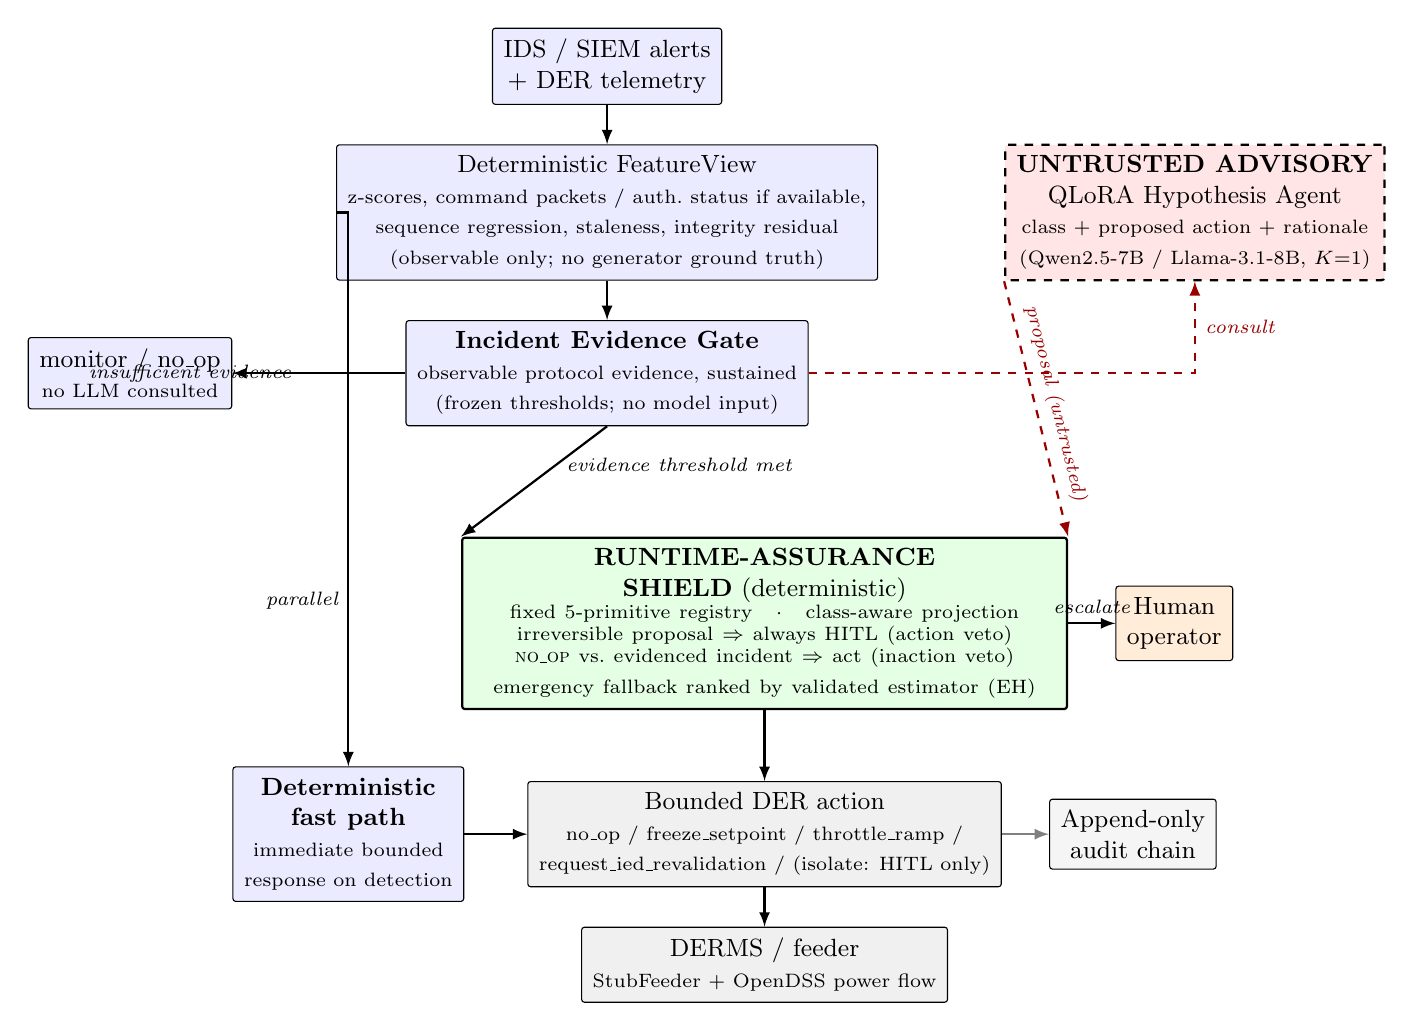
\begin{tikzpicture}[
  font=\small,
  node distance=5mm and 8mm,
  box/.style={draw, rounded corners=1pt, align=center, inner sep=4pt,
              minimum height=8mm},
  det/.style={box, fill=blue!8},
  llm/.style={box, fill=red!10, dashed, thick},
  shield/.style={box, fill=green!10, thick},
  phys/.style={box, fill=gray!12},
  lbl/.style={font=\scriptsize\itshape},
  arr/.style={-latex, thick},
]
% ---- left spine: deterministic decision path -------------------------
\node[det] (ids)  {IDS / SIEM alerts\\+ DER telemetry};
\node[det, below=of ids] (fv)   {Deterministic FeatureView\\
  \scriptsize z-scores, command packets / auth.\ status if available,\\
  \scriptsize sequence regression, staleness, integrity residual\\
  \scriptsize (observable only; no generator ground truth)};
\node[det, below=of fv] (gate) {\textbf{Incident Evidence Gate}\\
  \scriptsize observable protocol evidence, sustained\\
  \scriptsize (frozen thresholds; no model input)};
\node[det, left=22mm of gate] (noop) {monitor / no\_op\\
  \scriptsize no LLM consulted};
% ---- untrusted slow path ---------------------------------------------
\node[llm, right=16mm of fv] (qlora) {\textbf{UNTRUSTED ADVISORY}\\
  QLoRA Hypothesis Agent\\ \scriptsize class + proposed action + rationale\\
  \scriptsize (Qwen2.5-7B / Llama-3.1-8B, $K{=}1$)};
% ---- shield -----------------------------------------------------------
\node[shield, below=14mm of gate, xshift=20mm, text width=7.4cm] (shield)
 {\textbf{RUNTIME-ASSURANCE SHIELD} (deterministic)\\
  \scriptsize fixed 5-primitive registry \; $\cdot$ \; class-aware projection\\
  \scriptsize irreversible proposal $\Rightarrow$ always HITL (action veto)\\
  \scriptsize \textsc{no\_op} vs.\ evidenced incident $\Rightarrow$ act (inaction veto)\\
  \scriptsize emergency fallback ranked by validated estimator (EH)};
\node[box, right=6mm of shield, fill=orange!15] (hitl)
 {Human\\operator};
% ---- bottom: physical layer ------------------------------------------
\node[phys, below=9mm of shield] (act) {Bounded DER action\\
  \scriptsize no\_op / freeze\_setpoint / throttle\_ramp /\\
  \scriptsize request\_ied\_revalidation / (isolate: HITL only)};
\node[phys, below=5mm of act] (grid) {DERMS / feeder\\
  \scriptsize StubFeeder + OpenDSS power flow};
\node[det, left=8mm of act] (fast) {\textbf{Deterministic}\\\textbf{fast path}\\
  \scriptsize immediate bounded\\ \scriptsize response on detection};
% ---- audit ------------------------------------------------------------
\node[box, right=6mm of act, fill=gray!8] (audit) {Append-only\\audit chain};
% ---- edges ------------------------------------------------------------
\draw[arr] (ids) -- (fv);
\draw[arr] (fv) -- (gate);
\draw[arr] (gate) -- node[lbl, left, pos=0.6]{insufficient evidence} (noop);
\draw[arr] (gate.south) -- node[lbl, right, pos=0.35]{evidence threshold met}
  (shield.north west);
\draw[arr, dashed, red!60!black] (gate.east) -| node[lbl, right, pos=0.75]
  {consult} (qlora.south);
\draw[arr, dashed, red!60!black] (qlora.south west) --
  node[lbl, above, sloped]{proposal (untrusted)} (shield.north east);
\draw[arr] (shield) -- (act);
\draw[arr] (shield) -- node[lbl, above]{escalate} (hitl);
\draw[arr] (act) -- (grid);
\draw[arr] (fast) -- (act);
\draw[arr] (fv.west) -| node[lbl, left, pos=0.85]{parallel} (fast.north);
\draw[arr, gray] (act.east) -- (audit.west);
\end{tikzpicture}}

  \caption{\ours{} final architecture. Solid blue components are
    deterministic and own every decision that can reach the feeder; the
    dashed red component is the untrusted QLoRA advisory path, consulted
    only after the Incident Evidence Gate authorizes response under its
    frozen observable-evidence thresholds, and only able to select within the
    admissible candidate set the shield
    computes. A model-proposed irreversible primitive is never
    auto-executed. The deterministic fast path responds immediately in
    parallel; every executed action lands in an append-only audit chain.}
  \label{fig:architecture}
\end{figure*}

\subsection{Design rule and trust boundary}
\label{sec:method-layering}
\ours{} follows the runtime-assurance construction of
Simplex~\cite{Sha2001Simplex} and action
shielding~\cite{Alshiekh2018Shielding}: an unverified, high-capability
component may propose; a small deterministic, directly testable layer decides
what may execute. Three consequences structure the whole design
(Fig.~\ref{fig:architecture}). First, the LLM never emits executable
commands --- it selects from a fixed five-primitive registry
\{\textsc{no\_op}, \textsc{freeze\_\allowbreak setpoint},
\textsc{throttle\_\allowbreak ramp},
\textsc{request\_\allowbreak ied\_\allowbreak revalidation},
\textsc{isolate\_\allowbreak inverter}\}, so a
wrong output is a selection error, not arbitrary code execution. Second,
every quantity that can \emph{relax} a constraint is computed
deterministically from telemetry, never taken from model output; the
adversarial evaluation (\S\ref{sec:rq1}) shows why this rule is
load-bearing. Third, a deterministic fast path produces a bounded
response immediately, so consulting the model never delays containment.

\paragraph{Notation and invariants}
At tick $t$ the detector observes telemetry/packets $o_t$; a deterministic
FeatureView $\phi(o_{1:t})$ yields evidence state $e_t$ (\S\ref{sec:method-featureview}).
The Evidence Gate is a predicate $g(e_{1:t})\in\{0,1\}$
(\S\ref{sec:method-gate}). The registry is a fixed set
$\mathcal{A}=\{\textsc{no\_op},\textsc{freeze},\textsc{throttle},
\textsc{revalidate},\textsc{isolate}\}$ with irreversible subset
$\mathcal{I}=\{\textsc{isolate}\}$. The shield computes an admissible candidate set
$S(e_t)\subseteq\mathcal{A}$; the untrusted model proposes
$a^M_t\in\mathcal{A}\cup\{\bot\}$. The executed action is
$$
a^{\text{exec}}_t=\Pi\big(g(e_{1:t}),\,S(e_t),\,a^M_t,\,\tau_t\big),
$$
where $\Pi$ is the deterministic projection and $\tau_t$ the deadline state.
The design enforces, and we test, the following invariants (unit tests in
\texttt{test\_\allowbreak runtime\_\allowbreak safe\_\allowbreak gate.py} and
\texttt{test\_\allowbreak safety\_\allowbreak projection.py}):
\begin{enumerate}
\item[(I1)] $a^{\text{exec}}_t\in\mathcal{A}$ (only registry primitives execute);
\item[(I2)] $g(e_{1:t})=0 \Rightarrow a^{\text{exec}}_t=\textsc{no\_op}$ (gate closed $\Rightarrow$ monitor only);
\item[(I3)] $a^M_t\in\mathcal{I} \Rightarrow a^{\text{exec}}_t\notin\mathcal{I}$ without human approval (a model-proposed irreversible action is never autonomously executed);
\item[(I4)] if independent evidence $e_t$ establishes an incident, $a^M_t=\textsc{no\_op}$ cannot force $a^{\text{exec}}_t=\textsc{no\_op}$ (model inaction cannot veto evidenced response);
\item[(I5)] a late or failed model call leaves the deterministic fast-path action in force (the model can never \emph{prevent} the bounded response);
\item[(I6)] every proposal, veto, fallback, escalation, and execution is appended to the audit chain.
\end{enumerate}
I3 and I4 are the two-sided rule that model output may gate neither action
nor inaction; the evidence in $g$ and $S$ is computed deterministically,
so an attacker who controls the model's \emph{input or output} cannot
change it \emph{through the model}. This is independence from the LLM, not
robustness to a compromised network: an attacker able to inject or forge
unauthenticated protocol traffic can still move the gate by manufacturing
observable evidence (\S\ref{sec:bg-trust}), which is why the architecture
escalates irreversible actions to a human rather than trusting any single
evidence source. These invariants are deterministic and directly testable;
we do not claim a formal proof.

``Trustworthy'' in this paper denotes implemented, measured properties
--- bounded action generation, schema compliance, containment within the
tested adversarial suite, human oversight, auditability, consequence
awareness, conservative fallback --- not a formal guarantee. The supplementary
material maps each property to its mechanism, the experiment that evaluates it,
and its remaining limitation.

\subsection{Deterministic FeatureView}
\label{sec:method-featureview}
A deterministic first stage converts the rolling telemetry/event window
into a structured FeatureView. Every feature is computed from quantities
observable on the wire or from the defender's grid model, never from
attacker-set ground truth. Table~\ref{tab:provenance} lists each feature,
its observable source, and the attacker's influence over it. The features
are: per-asset z-scores against a 60-step baseline; voltage-band
excursion; a forged-command-packet count; a duplicate-payload signature;
a persistent-freeze flag; a SCADA staleness signature (consecutive
samples whose reported timestamps fail to advance --- the fingerprint of
replay and denial-of-service, which re-emit captured frames); a protocol
sequence-number regression (a frame carrying a sequence number below the
running high-water mark --- the wire-visible signature of replay); and a
telemetry-integrity residual (a reported power above the asset's rated
capacity, physically impossible and therefore a corrupted reading ---
the observable signature of a high-magnitude false-data-injection
attack). No feature is read from attacker-set ground truth; a provenance
audit (Table~\ref{tab:provenance}) records, for each feature, its
observable source and the attacker's influence over it, and we report the
detectability this observable-only discipline permits --- and the FDI
limit it exposes --- in \S\ref{sec:rq2}\@. Every downstream stage, including the LLM prompt,
consumes this single numeric grounding; severity is a bounded
deterministic score, not a model output.

% Table 3: trust boundary and evidence provenance.
% Page-breaking xltabular so the tall table never overflows into the page footer.
{\footnotesize
\begin{xltabular}{\textwidth}{@{}>{\raggedright\arraybackslash}p{0.19\textwidth}
 >{\raggedright\arraybackslash}p{0.22\textwidth}
 >{\raggedright\arraybackslash}p{0.13\textwidth}
 >{\raggedright\arraybackslash}X@{}}
\caption{Evidence provenance and trust boundary for the runtime FeatureView.
Every runtime feature is computed from wire-observable telemetry/packets or
the defender's grid model; generator ground-truth flags are excluded by design
(last row). Wire-observable is not authenticated: an attacker able to inject
unauthenticated traffic can forge much of this evidence, so it is robust to a
compromised model but not a compromised network. ``Attacker influence'' is the
attacker's ability to forge or suppress the feature.}\label{tab:provenance}\\
\toprule
Feature & Observable source & Attacker influence & Runtime use / failure mode \\
\midrule
\endfirsthead
\multicolumn{4}{@{}l}{\emph{Table~\ref{tab:provenance} (continued)}}\\[2pt]
\toprule
Feature & Observable source & Attacker influence & Runtime use / failure mode \\
\midrule
\endhead
\midrule
\multicolumn{4}{r@{}}{\emph{continued on next page}}\\
\endfoot
\bottomrule
\endlastfoot
Command-packet count & DNP3/IEC-61850 command frame on the wire & Can forge command frames & Opens gate; forged commands indistinguishable from legitimate ones absent authentication (benign-command discrimination is a stated limit) \\
\addlinespace[2pt]
Duplicate-payload signature & Repeated identical frame payloads & Can inject duplicates & Replay/echo signature; benign historian echo is an irreducible ambiguity \\
\addlinespace[2pt]
Staleness (non-advancing timestamp) & Frame reported-time field & Can freeze/replay timestamps & DoS/replay signature; a re-timestamped replay evades it (caught instead by sequence regression) \\
\addlinespace[2pt]
Sequence regression & IEC-61850 sqNum / DNP3 sequence vs.\ running high-water mark & Cannot lower a delivered seq without detection unless it also spoofs the counter end-to-end & Replay signature; observable, not authenticated \\
\addlinespace[2pt]
Integrity residual & Reported power vs.\ rated capacity (defender grid model) & Bounded: a value above capacity is physically impossible & High-magnitude FDI; \emph{sub-capacity FDI is not observable here} (documented miss) \\
\addlinespace[2pt]
Persistent freeze & $\ge$10 consecutive zero-power samples & Can force zero output & DoS signature \\
\addlinespace[2pt]
Per-asset z-score, voltage band & Reported power / bus voltage & Can bias reported power (soft) & Soft evidence; not separable from benign transients, so not used to open the gate alone \\
\midrule
\textbf{Excluded by design:} any generator ground-truth flag & \emph{e.g.\ an injector \texttt{tampered} bit} & \emph{fully attacker-/generator-set; an oracle} & \textbf{Never read by the runtime}; unit tests confirm no such field enters a feature \\
\end{xltabular}
\par}


\subsection{Incident Evidence Gate}
\label{sec:method-gate}
The shield constrains \emph{which} action may execute, but our earlier
evaluation showed it had no mechanism for deciding that \emph{no}
incident exists: on benign stochastic days, cloud transients and
measurement noise pushed the pipeline into unnecessary mitigation on
every episode (\S\ref{sec:rq2}). The Evidence Gate closes this gap
deterministically. It opens only when \emph{sustained protocol-level
evidence} --- itself wire-observable and, absent authentication, forgeable
by a network attacker (\S\ref{sec:bg-threat}): a forged command packet, a
duplicate-payload/sequence
regression (replay), non-advancing timestamps or a persistent zero-freeze
(DoS), or a rating-plausibility integrity residual (high-magnitude FDI),
all observable (Table~\ref{tab:provenance}) --- is sustained for the
calibrated persistence window. A physical-only (z-score/voltage) path
exists but its calibrated persistence threshold effectively disables it:
on the development split, no physical-only setting separated attacks from
benign PV transients without either missing attacks or admitting benign
days, which is itself a finding about DER telemetry --- and, after the
observable-only evidence set, is the reason a \emph{sub-capacity} FDI (whose only trace
is such a physical deviation) is not reliably separable from benign
operation without redundant sensing (\S\ref{sec:rq2}). While the gate is
closed the system monitors; no mitigation executes and \emph{the LLM is
not consulted}, which also removes the model's exposure to benign-day
prompt content. Thresholds are calibrated on a development split and
frozen before the held-out evaluation; the gate reads no model output.

\subsection{Untrusted advisory path}
\label{sec:method-advisory}
When the gate opens, a QLoRA-adapted~\cite{Dettmers2023_QLoRA} open-weights
backbone (Qwen2.5-7B~\cite{Hu2024_Qwen25} or
Llama-3.1-8B~\cite{Dubey2024_Llama31}, NF4 4-bit on a single RTX~3080) receives the compact
FeatureView prompt and returns a JSON hypothesis: attack class, affected
asset, confidence, rationale, proposed action. Serving is strict: a run
aborts if the intended backbone or adapter is not loaded, and every call
records the adapter SHA-256, prompt hash, raw output, parse status and
latency, so no deterministic fallback can masquerade as a model result:
a silent fallback would invalidate any claim about model behaviour, so it
is made impossible by construction rather than assumed absent.
At each eligible gated decision tick the advisory path draws one greedy
generation ($K{=}1$); a sustained incident may therefore trigger repeated
consultations across ticks (the per-configuration call counts in
Table~\ref{tab:holdout-v3}). Here $K$ is the number of generations \emph{per
consultation} for self-consistency, not the number of consultations per
incident: $K{=}1$ draws one generation, $K{=}3$ draws three. The default is
$K{=}1$; $K{=}3$ was removed after measurement showed it tripled latency without
a decision-quality gain that survives the shield. Fine-tuning uses a 200-example
DER/ICS corpus with assistant-turn loss masking (supplementary material).

\subsection{Runtime-assurance shield}
\label{sec:method-shield}
The shield computes, deterministically, the \emph{admissible candidate set}
for the current situation and lets the model choose only within it.
Removals are recorded per decision: actions inappropriate for the
evidence class (a telemetry-layer compromise must not be answered by
physically disconnecting a healthy asset), actions ineffective against
the mechanism, and all non-\textsc{no\_op} actions when severity is
below threshold. Two rules are absolute. (i)~A model-proposed
\emph{irreversible} primitive (\textsc{isolate\_inverter}) is never
auto-executed: where the evidence class admits it as a candidate at all it
escalates to a human operator, and where the class forbids it the shield
vetoes it and falls back deterministically
(Table~\ref{tab:action-policy}). An earlier
variant gated this on model-stated confidence and was falsified by
adversarial evaluation --- injected prompts manufacture exactly the
confidence the gate keyed on, making that variant worse than no shield
(\S\ref{sec:rq1}). Attacker-influenceable quantities do not
relax constraints. (ii)~When the model's proposal is unusable ---
invalid, out of registry, below the confidence floor, or vetoed --- the
shield falls back deterministically, ranking the admissible candidate set with the
horizon-aware impact estimator described next.
Table~\ref{tab:action-policy} states the complete frozen policy per evidence
class --- which actions may execute autonomously, which are escalation-only,
which are removed and why, and the deterministic fallback order --- together
with the testbed action semantics and recovery condition. The policy is
author-specified: the evaluation establishes conformance to this stated
policy, not an independent validation of its operational correctness or
completeness.

\begin{table}[t]
\centering\small
\caption{Frozen class-aware action policy of the shield (source of truth:
\texttt{safety\_projection.py}; machine-readable export
\texttt{code/configs/action\_policy.yaml}, verified by
\texttt{tests/test\_action\_policy.py}). Actions: N = \textsc{no\_op},
F = \textsc{freeze\_setpoint}, T = \textsc{throttle\_ramp}, R =
\textsc{request\_ied\_revalidation}, I = \textsc{isolate\_inverter}
(irreversible). \emph{Autonomous} actions may execute without a human; a
model-proposed I is never auto-executed --- escalated to a human where the
class admits it (I3), vetoed with deterministic fallback where it does not
--- and the deterministic fallback never selects it. Non-N actions require
severity $\geq 0.30$; honouring a model choice requires stated confidence
$\geq 0.40$. Removals: inappr.\ = class-inappropriate, ineff.\ =
mechanism-ineffective. Testbed semantics: F holds the last validated
setpoint (70\% of rated kW) for the episode remainder; T restricts ramping
to the IEEE\,1547 minimum; I is absorbing and requires operator
restoration. No automatic release is modelled: stand-down requires the
gate's sustained evidence to clear and an operator/DERMS resume, never
model output alone (I4). The policy is author-specified, motivated by the
class mechanism and counterfactual rollouts; the evaluation establishes
conformance to it, not its independent operational validation.}
\label{tab:action-policy}
\footnotesize\setlength{\tabcolsep}{4pt}
\begin{tabular}{lllll}
\toprule
Evidence class & Autonomous & Escalation-only & Removed & Fallback \\
\midrule
Command spoof & N, F, T & I & R\,(ineff.) & F$\rightarrow$T$\rightarrow$N \\
Replay & N, F, T, R & --- & I\,(inappr.) & R$\rightarrow$F$\rightarrow$N \\
DoS & N, F & I & T,R\,(ineff.) & F$\rightarrow$N \\
FDI (rating residual) & N, F, R & --- & T\,(ineff.); I\,(inappr.) & F$\rightarrow$R$\rightarrow$N \\
No evidence / benign & N & --- & F,T,R,I\,(inappr.) & N \\
\bottomrule
\end{tabular}
\end{table}


\subsection{Horizon-aware impact estimator (EH)}
\label{sec:method-estimator}
The original estimator integrated per-action cost over a fixed 60\,s
window. Counterfactual validation --- branching the simulator at the
decision instant and executing every candidate under identical exogenous
trajectories --- showed it selected a tie-optimal action in only a third of
configurations (Table~\ref{tab:eh-v3}): over the true incident horizon,
candidates differ by two orders of magnitude more than over 60 seconds, so a
60\,s ranking is usually wrong. The repaired estimator EH uses only
decision-time information: a deterministic class-family hypothesis from
protocol evidence (spoof-like, FDI-like, or stale, the latter because
replay and DoS are indistinguishable at decision time), a
remaining-horizon estimate from a development-calibrated mean-residual-life prior,
and restoration-horizon accounting for absorbing actions such as
isolation. The true attack end time is never an input. EH is retained in
the architecture only because it passed a hash-frozen held-out
holdout (\S\ref{sec:rq3}); its point predictions remain
imprecise, so it is used to \emph{rank} the admissible candidate set, never to claim
impact magnitudes.

\subsection{Fast path, slow path, oversight, audit}
\label{sec:method-deployment}
The deterministic fast path (FeatureView $\rightarrow$ evidence class
$\rightarrow$ bounded primitive) responds within one control tick. The
model path is a slow path under an explicit service-level objective:
measured consultation latency (${\approx}5.5$\,s at $K{=}1$ on the reference GPU)
means the model contributes within a 15\,s SLO and is skipped ---
without loss of containment --- under tighter deadlines
(\S\ref{sec:rq4}). Escalations carry the model's proposal,
rationale and the shield's veto reasons to the operator. Every decision
appends to a SHA-256 hash-chained audit record. Relative to a trusted stored
chain head, verification detects modification, deletion, and reordering of
records; it does not provide origin authentication, trusted timestamping, or
protection against complete recomputation by an attacker who controls the entire
log. Full prompts, schemas,
state-machine contracts, and protocol examples are in the supplementary
material.

\section{Experiments}
\label{sec:eval}

\subsection{Evaluation design}
\label{sec:exp-design}
The runtime path throughout is \emph{runtime-safe}: every feature is computed
only from wire-observable telemetry, packets, and the defender's rated-capacity
model (Table~\ref{tab:provenance}); no feature reads attack ground truth. Real
QLoRA adapters (Qwen2.5-7B, Llama-3.1-8B; NF4 4-bit on one RTX~3080) run under
strict serving --- any run whose backbone or adapter is not loaded, whose
provenance is missing, or that would fall back to a heuristic, aborts. Ground
truth is used only by the offline evaluator after an action is chosen. The
unit of statistical inference is the \emph{configuration}; genuine stochastic
episodes are averaged within a configuration. Binary paired outcomes use the
exact McNemar test; continuous outcomes use paired sign-flip permutation tests
with paired bootstrap 95\% CIs and Cohen's $d_z$, Holm-corrected within each
hypothesis family; the permutation and bootstrap resampling draws are shared
across the contrasts of a family (common random numbers), so identical paired
difference vectors receive identical intervals; zero-event rates carry a
Clopper--Pearson 95\% upper bound.

Frozen assets, each hash-pinned before use: a canonical \textbf{70-case}
adversarial suite (14 families $\times$ 5 held-out cases per backbone,
leakage-controlled against the 200-example fine-tuning corpus --- zero exact or
normalized duplicates); a \textbf{32-configuration} Evidence-Gate test set plus
per-magnitude FDI probes; a hash-frozen \textbf{49-configuration} end-to-end holdout (33 attack across four families
plus fleet, 16 benign; two feeders; three episodes each) used for
system evaluation only; and a \textbf{12-configuration} estimator holdout for
counterfactual validation. A separate 25-configuration library is used for
development and threshold selection only, never for held-out reporting.
IEEE-123 is unavailable in the repository; the
holdout uses IEEE-13/34 and states the reduced feeder scope rather than
substituting.

\subsection{RQ1: does adversarial output reach an unsafe executable action?}
\label{sec:rq1}
\emph{Experiment.} Each of eight arms faces the canonical 70-case suite as
sustained input (eight ticks, so persistence-gated components fire), on the
runtime-safe architecture. The arms share the frozen case definitions, but
model generation is performed independently within each arm --- no arm
replays another arm's model output. Arm-level comparisons therefore
characterise complete-system behaviour and do not estimate a matched causal
effect on identical frozen model outputs. Per-decision provenance records the
model's proposal and the executed action separately; the denominator is the
adversarial case.

\emph{Result} (Table~\ref{tab:adv-v3-qwen}, Fig.~\ref{fig:containment-v3}). The
model is genuinely consulted --- it proposes a non-\textsc{no\_op} action --- on
$64/70$ cases (Qwen) and $70/70$ (Llama), so the containment below is the shield
acting on real proposals, not non-consultation. The unshielded model executes the
irreversible \textsc{isolate\_inverter} primitive on $61$ of $70$ cases (Qwen;
irreversible-execution rate $0.871$) and $18$ of $70$ (Llama; $0.257$); the
distinct, broader forbidden-action rate (any action in the case's must-not set)
is $46/70=0.657$ for Qwen. The full architecture,
and every ablation arm that retains the class-aware avoidance, executes it
\emph{zero} times (Clopper--Pearson 95\% upper bound $0.051$; policy violation
$0.000$). The independently executed arm without class-aware avoidance
exhibits $36$ of $70$ (Qwen) and $37$ of $70$ (Llama) executions (violation
$0.443$/$0.357$). The arm without the Evidence Gate shows unchanged
adversarial containment (still zero) --- the shield handles consulted
proposals regardless; the gate's role is benign-day selectivity (RQ2). The confidence-gated variant, which admitted an irreversible
action when model-stated confidence cleared a threshold, was \emph{worse than no
shield} ($0.743$ versus $0.657$ unshielded) because injection prompts manufacture that
confidence.

\emph{Interpretation.} Exactly one mechanism carries adversarial containment:
deterministic removal of unsafe actions, with irreversible proposals always
escalated. The consistency of the unshielded-model figure with an independent earlier
suite (61/70) is a cross-check on the harness. \emph{Limitation.} Marginal
contributions are measured against this suite; a component idle here may matter
elsewhere, and suite-bounded zeros are not universal guarantees.

\emph{Structural verification.} Because the 70-case suite only \emph{samples}
the danger, we additionally verify the shield structurally: we exhaustively
enumerate the discretised decision state space of the deterministic projection
--- $40{,}824$ combinations of evidence class, model proposal (including
out-of-registry and malformed output), stated confidence, severity, parse
status, and protocol-evidence hint --- and check every safety property at every
point. The executed action is always in the fixed registry, the irreversible
primitive is never executed autonomously (vetoed or escalated, never
executed), no class-inappropriate
action executes, a model stand-down never vetoes a deterministically evidenced
incident, and model failure always yields the deterministic fallback: $0$
violations over all $40{,}824$ points. Mutation tests confirm the properties are
load-bearing, not vacuous --- disabling the irreversible-escalation, class-aware
avoidance, or inaction-veto guard produces $1008$, $144$, and $3930$ violations
respectively. This is exhaustive over the modelled state space rather than a
sample from a real attack population.

\input{tables/final_v3/table_adversarial_v3_qwen}
\begin{table}[t]\centering\small
\caption{Canonical 70-case adversarial containment (llama), sustained input, observable-only runtime. Denominator = adversarial case ($n{=}70$). \emph{Irrev.\ prop.}\ and \emph{Irrev.\ exec.}\ are the irreversible-proposal and irreversible-\emph{execution} counts (action $=$ \texttt{isolate\_inverter}); \emph{Forbidden act.}\ is the distinct forbidden-action count (executed action in the case's must-not set). Zero-execution arms carry a two-sided Clopper--Pearson 95\% upper bound (\emph{exec.\ up95}). The correct-refusal rate and full per-arm metrics are in the supplementary material.}
\label{tab:adv-v3-llama}
\resizebox{\columnwidth}{!}{%
\begin{tabular}{lccccc}
\toprule
Arm & $n$ & Irrev.\ prop. & Irrev.\ exec. & exec.\ up95 & Forbidden act. \\
\midrule
Full arch. & 70 & 37/70 & 0/70 & 0.051 & 0/70 \\
$-$Evidence gate & 70 & 62/70 & 0/70 & 0.051 & 0/70 \\
$-$Projection & 70 & 37/70 & 0/70 & 0.051 & 0/70 \\
$-$Class avoidance & 70 & 37/70 & 37/70 & 0.649 & 25/70 \\
$-$Caution/HITL & 70 & 37/70 & 0/70 & 0.051 & 0/70 \\
$-$EH fallback & 70 & 37/70 & 0/70 & 0.051 & 0/70 \\
Deterministic only & 70 & 0/70 & 0/70 & 0.051 & 0/70 \\
Unshielded & 70 & 18/70 & 18/70 & 0.376 & 18/70 \\
\bottomrule
\end{tabular}}
\end{table}


\begin{figure}[t]
  \centering
  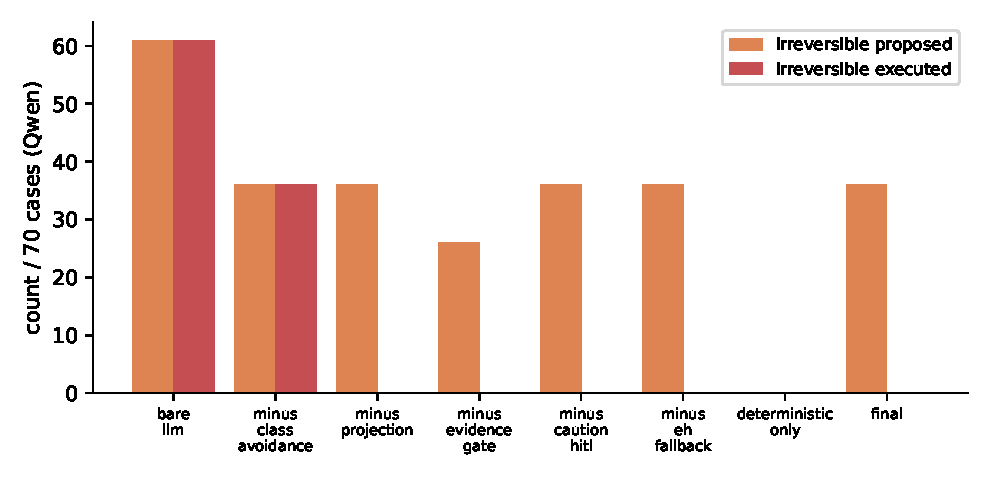
\includegraphics[width=0.95\columnwidth]{figure/final_v3/fig_containment_v3.pdf}
  \caption{Irreversible actions proposed versus executed per arm on the
    canonical 70-case runtime-safe adversarial suite (Qwen). Arms are
    executed independently on the shared frozen case definitions
    (\S\ref{sec:rq1}). The full architecture and every avoidance-retaining
    ablation arm execute zero; the arm without class-aware avoidance
    exhibits execution; the unshielded comparator executes 61/70.}
  \label{fig:containment-v3}
\end{figure}

\subsection{RQ2: does the gate reduce benign response yet retain incidents?}
\label{sec:rq2}
\emph{Experiment.} Gate thresholds are calibrated on development data and
hash-frozen before a one-shot evaluation on the 32-configuration test set plus
per-magnitude FDI probes, all runtime-safe. We report gate-open coverage per
family (did the gate fire during the attack --- a detector-side quantity,
distinct from downstream correct mitigation) and benign false-open, with
Clopper--Pearson intervals.

\emph{Result} (Table~\ref{tab:gate-v3}, Fig.~\ref{fig:gate-v3}). Under the
observable-only feature set, the tested gate rules opened in all four tested
configurations of each of command-spoof, replay (sequence regression), and DoS
(timestamp staleness) --- each $4/4$ --- and in the single tested above-capacity
FDI probe ($1/1$, caught by the rating-plausibility residual). These are small
samples and the Clopper--Pearson intervals (Table~\ref{tab:gate-v3}) remain wide;
they are not population-level detection estimates. Benign false-open is
$4/16 = 0.25$ $[0.07, 0.52]$, of which three of four are the historian-echo
protocol ambiguity. The honest cost is explicit: sub-capacity FDI is missed ($0/1$
medium, $0/1$ low) --- it has no observable hard signature and cannot be
separated from benign transients without redundant sensing, so we report FDI
coverage split by magnitude rather than as one number. On the 16 benign holdout
configurations, an exact McNemar test found no significant difference in
benign false-action between the deterministic path (D0) and the oracle-projection
arm (discordant pairs $4/0$, $p=0.125$). The gate's measured benefit is instead
that it cuts benign-day model consultations (\S\ref{sec:disc-timing}), bounding
the model's exposure to attacker-controllable prompt content.

\emph{Command evidence requires authentication.} A command packet on the
wire is not proof of an attack: a forged command and a legitimate DERMS
command are observationally identical unless the command is authenticated.
We make the distinction explicit (Table~\ref{tab:gate-auth}) by evaluating
command-spoof detection and benign \emph{legitimate authenticated command
bursts} under three policies. Treating any command as an attack detects the
spoof ($3/3$) but false-opens on every legitimate burst ($2/2$); requiring a
failed-authentication check detects the forgery ($3/3$) and does not
false-open ($0/2$); without authentication the command is \emph{UNKNOWN}
evidence and the gate can rely only on a separate protocol signature --- here
the duplicate-payload signature, which also false-opens because repeated
legitimate commands trip it. The lesson is that command-based detection is
sound only with authenticated command evidence or an explicit UNKNOWN
outcome routed to a human; we implement no cryptographic check and therefore
report command-spoof coverage under the observable-only regime as
conditional on this assumption.

\emph{Interpretation.} The tested gate rules detected the evaluated instances
that contained their prespecified observable protocol signatures (command-spoof,
replay, DoS); the fourth family (sub-capacity FDI) has no such signature and is
an observability limit, and command-based detection carries the authentication
caveat above. These are small tested samples, not population-level detectability
claims. \emph{Limitation.} The gate assumes an
instrumented protocol layer; a full DNP3/IEC-61850 sequence state machine
(reset, wrap, retransmission, session restart) and cryptographic
authentication are modelled only in part, and a stealthy attacker forging
internally consistent authenticated evidence is out of scope.

\begin{table}[t]
\centering\small
\caption{Evidence Gate detector-side coverage: per-group gate-open and benign
false-open on the hash-frozen 32-configuration test set plus per-magnitude FDI
probes, using only observable evidence. Thresholds calibrated on development
data and frozen before this evaluation. Two-sided Clopper--Pearson 95\%
intervals. Sub-capacity FDI (medium/low) has no observable hard signature and
is reported as a coverage miss.}
\label{tab:gate-v3}
\begin{tabular}{lccc}
\toprule
Group & $k/n$ & Rate & 95\% CI \\
\midrule
Benign false-open & 4/16 & 0.25 & [0.07, 0.52] \\
Gate-open command-spoof & 4/4 & 1.00 & [0.40, 1.00] \\
Gate-open DoS & 4/4 & 1.00 & [0.40, 1.00] \\
Gate-open FDI (high) & 1/1 & 1.00 & [0.03, 1.00] \\
Gate-open FDI (low) & 0/1 & 0.00 & [0.00, 0.97] \\
Gate-open FDI (med) & 0/1 & 0.00 & [0.00, 0.97] \\
Gate-open replay & 4/4 & 1.00 & [0.40, 1.00] \\
\bottomrule
\end{tabular}
\end{table}

\begin{table}[t]\centering\small
\caption{Command evidence requires authentication. Gate-open outcome for command-spoof attacks (forged, failed authentication) and benign \emph{legitimate authenticated command bursts}, under three command-evidence policies (three configurations each, any-episode aggregation). Only requiring a failed-authentication check both detects the forgery and does not false-open on legitimate commands; treating any command as an attack, or having no authentication (command evidence UNKNOWN, so only physical corroboration counts --- here the duplicate-payload of repeated legitimate commands), false-opens.}
\label{tab:gate-auth}
\begin{tabular}{lcc}
\toprule
Command-evidence policy & Spoof gate-open & Benign false-open \\
\midrule
Any command $=$ attack & 3/3 & 2/2 \\
Require failed auth. & 3/3 & 0/2 \\
Unauthenticated (UNKNOWN) & 3/3 & 2/2 \\
\bottomrule
\end{tabular}
\end{table}


\begin{figure}[t]
  \centering
  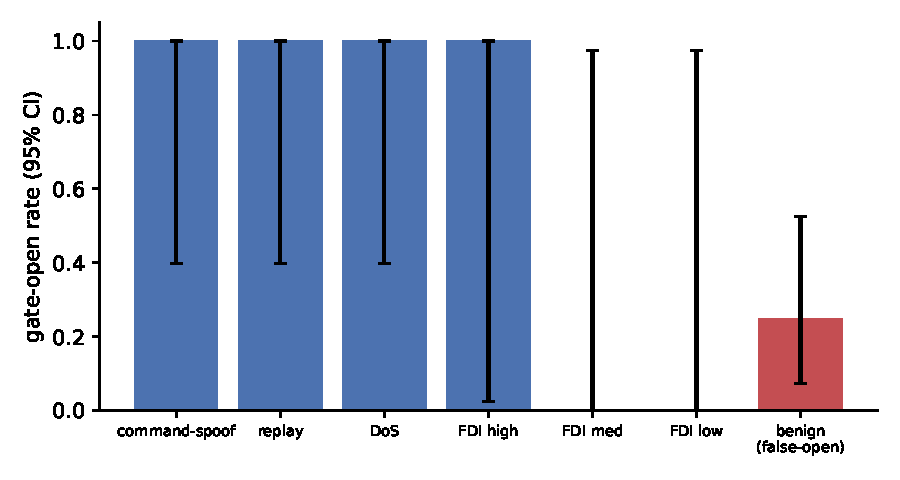
\includegraphics[width=0.82\columnwidth]{figure/final_v3/fig_gate_v3.pdf}
  \caption{Runtime-safe gate-open rate by attack family and benign false-open
    (95\% Clopper--Pearson intervals), using only observable evidence.
    Sub-capacity FDI (medium/low) is a documented observability miss.}
  \label{fig:gate-v3}
\end{figure}

\subsection{RQ3: what physical cost remains on an independent holdout?}
\label{sec:rq3}
\emph{Experiment.} The hash-frozen 49-configuration holdout (opened once, never
used for tuning) runs eight arms under the runtime-safe architecture with real
adapters: the deterministic fast path (D0); the ungated, fixed-cadence
model-only arms (ModelOnly-Q/L); the class-override shield (ClassOnly-Q/ClassOnly-L); the corrected projection
(SafeProj-Q/SafeProj-L) with irreversible-escalation, inaction-veto, and EH-ranked
fallback; and the oracle-class projection (OracleClass-Proj) as an evaluator-only upper
bound. Configuration is the inference unit.

\emph{Result} (Table~\ref{tab:holdout-v3}, Fig.~\ref{fig:holdout-v3},
Table~\ref{tab:stats-primary}). Zero serving fallbacks; adapters verified per
call. Mean attack ENS is D0 $0.352$, SafeProj-Q $0.537$, SafeProj-L $0.750$, ClassOnly-Q
$4.006$, ClassOnly-L $4.749$, ModelOnly-Q/L $8.484$, and OracleClass-Proj $0.067$.
The ModelOnly arms are \emph{diagnostic rather than matched shield ablations}:
they are ungated and poll the model on a fixed cadence that typically misses the
short attack window, so neither executes an effective mitigation in this holdout.
Their identical physical outcomes (byte-identical for ModelOnly-Q and ModelOnly-L,
both executing zero actions) therefore reflect the common unmitigated trajectory
rather than identical model behaviour, and their high ENS is \emph{not} a causal
estimate of shield removal --- shield use, evidence delivery, consultation
timing, and policy all differ at once. The evidence for unsafe unshielded
\emph{execution} is the adversarial result of \S\ref{sec:rq1}, where the model is
given the attack evidence directly. The projection arms show \emph{no
statistically detectable difference} from the deterministic path (SafeProj-Q
$+0.19$\,kWh, SafeProj-L $+0.40$\,kWh, both Holm $p=1.0$); no equivalence margin
was pre-registered, so we claim only the absence of a detectable difference, not
equivalence.
The ground-truth-class oracle is \emph{modestly better} than the deterministic
path (OracleClass-Proj$-$D0 $=-0.285$\,kWh, 95\% CI $[-0.69, -0.05]$, $d_z=-0.27$, raw
$p=0.015$; Holm-adjusted $p=0.11$, so the improvement does not survive
multiplicity correction across the primary family). We report this as a modest,
not-significant benefit rather than either ``no difference'' or a significant
gain: the bootstrap interval excludes zero while the adjusted test does not, a
distinction we make explicit. The LLM advisers do not reproduce even this
modest oracle benefit. Benign false-action is $0.062$ for the shielded model
arms against $0.25$ for the ungated deterministic path. That these conclusions
hold on prespecified, hash-frozen held-out configurations, under a runtime that
reads no attack ground truth, is the evidence they are not artefacts of a
strong detector.

\emph{Static OpenDSS power-flow plausibility check.} The 49-configuration
comparison uses the StubFeeder, a fast, stochastic simulation we treat as a
diagnostic rather than a deployment-validity result. To check that its physical
readings are plausible, we re-ran the deterministic and oracle-projection arms
through static OpenDSS IEEE-13/34 AC power-flow snapshots on the pre-registered
12-configuration subset, under the same observable-only runtime: all solves
converged (zero non-converged), and the two arms behave near-identically (mean
curtailment $17.6$ vs $17.7$\,kWh over the 11 attack configurations --- the
twelfth is the benign control --- and minimum voltage $0.975$\,pu). ENS is zero on
this subset because the feeders remain within the served-load envelope, so the
meaningful observed quantities are curtailment and voltage, not ENS. This is a
static snapshot check, not a dynamic quasi-static time-series study and not
real-feeder or utility validation; StubFeeder results remain simulation-based
diagnostic evidence. \emph{Limitation.} A dynamic quasi-static time-series study
across all arms is future work.

The estimator that ranks the shield's fallback set is validated separately
(Table~\ref{tab:eh-v3}): against branched counterfactual rollouts on the frozen
estimator holdout, the legacy 60-second estimator selects a tie-aware optimal
action in only a third of nominal configurations (top-1 $0.33$; $0.40$ averaged
over the ten robustness conditions) and carries large regret when it errs
(mean $76.3$\,kWh-eq), while the horizon-aware EH
selected a zero-regret action in all 12 tested held-out configurations and
retained that ranking under the evaluated perturbations (horizon misspecification
$\pm50\%$, delayed and partial execution, alternative cost weights). This result
reflects the coarse, structurally determined five-action ordering and the small
holdout; it should not be read as evidence of accurate impact-magnitude
prediction (MAE $\approx26$\,kWh) or of general real-feeder robustness, and we
make no magnitude-prediction claim.

\emph{Interpretation.} After containment, the residual physical cost of
consulting the model is small and is dominated by safe-but-suboptimal proposals
the shield honours inside the admissible candidate set --- a bounded, backbone-dependent cost the
admissible-set design, not the model, determines. \emph{Limitation.} StubFeeder and
static/quasi-static OpenDSS physics; the OpenDSS power-flow check
(supplementary material) is static, not dynamic.

\begin{table}[t]
\centering\small
\caption{Held-out end-to-end evaluation: 49 configurations (33 attack, 16
benign) $\times$ 3 stochastic episodes, observable-only runtime.
Configuration is the inference unit; episodes averaged within configuration.
\emph{Closed-loop coverage} is whether the incident is flagged at any tick of
the attack window in the closed loop; it is arm-dependent because each arm's
action feeds back into telemetry and the sustained-evidence gate (e.g.\ time to
first gate-open is $20$\,s for D0 vs.\ $111$\,s for L1), and is \emph{N/A} for
the ungated bare arms. It is \emph{not} the deterministic pre-action gate, which
is model-independent and identical across arms for identical input (verified:
$11{,}020$ pre-action ticks, $0$ violations); the detector-side gate recall is
Table~\ref{tab:gate-v3}. \emph{LLM calls} = sum over the 33 attack configs of
per-config mean calls (a sustained incident re-consults across ticks). Benign
false-action (FA) is physical-side. LLM arms run under strict serving (zero
fallbacks). Paired statistics in Table~\ref{tab:stats-primary}.}
\label{tab:holdout-v3}
\begin{tabular}{lcccccc}
\toprule
Arm & ENS & Curt. & Closed-loop & Benign & LLM & HITL \\
 & (kWh) & (kWh) & coverage & FA rate & calls & \\
\midrule
D0 & 0.352 & 11.52 & 0.949 & 0.250 & 0 & 0 \\
ModelOnly-Q & 8.484 & 17.05 & N/A & 0.000 & 66 & 0 \\
ModelOnly-L & 8.484 & 17.05 & N/A & 0.000 & 66 & 0 \\
ClassOnly-Q & 4.006 & 13.48 & 0.657 & 0.000 & 167 & 0 \\
ClassOnly-L & 4.749 & 13.84 & 0.657 & 0.062 & 167 & 0 \\
SafeProj-Q & 0.537 & 11.85 & 0.657 & 0.062 & 143 & 44 \\
SafeProj-L & 0.750 & 12.01 & 0.495 & 0.062 & 143 & 0 \\
OracleClass-Proj & 0.067 & 11.65 & 0.960 & 0.000 & 0 & 0 \\
\bottomrule
\end{tabular}
\end{table}

\begin{table}[t]
\centering\small
\caption{Primary paired configuration-level comparison on the held-out
49-configuration set: attack-window ENS difference of each arm minus the
deterministic fast path (D0), episodes averaged within configuration. Paired
bootstrap 95\% CI, Cohen's $d_z$, paired sign-flip permutation $p$, and
Holm-adjusted $p$ across this primary family; resampling draws are shared
across contrasts (common random numbers), so identical difference vectors
receive identical intervals (ModelOnly-Q/L). ``*'' marks Holm $p<0.05$. The
bootstrap CI can exclude zero while the adjusted test does not (OracleClass-Proj),
which we report as a modest, not-significant effect. ModelOnly arms are
diagnostic, not matched shield ablations (\S\ref{sec:rq3}).}
\label{tab:stats-primary}
\begin{tabular}{lcccccc}
\toprule
Contrast (ENS) & Mean diff & 95\% CI & $d_z$ & $N$ & $p_{\text{raw}}$ & $p_{\text{Holm}}$ \\
 & (kWh) & (kWh) & & cfg & & \\
\midrule
ModelOnly-Q$-$D0 & +8.133 & [+4.25, +12.46] & +0.66 & 33 & $<$0.001 & 0.008\,* \\
ModelOnly-L$-$D0 & +8.133 & [+4.25, +12.46] & +0.66 & 33 & $<$0.001 & 0.008\,* \\
ClassOnly-Q$-$D0 & +3.654 & [+1.31, +6.35] & +0.49 & 33 & 0.015 & 0.107 \\
ClassOnly-L$-$D0 & +4.398 & [+1.96, +7.12] & +0.57 & 33 & 0.005 & 0.041\,* \\
SafeProj-Q$-$D0 & +0.186 & [-0.62, +1.33] & +0.06 & 33 & 1.000 & 1.000 \\
SafeProj-L$-$D0 & +0.398 & [-0.47, +1.64] & +0.13 & 33 & 0.727 & 1.000 \\
OracleClass-Proj$-$D0 & -0.285 & [-0.69, -0.05] & -0.27 & 33 & 0.015 & 0.107 \\
\bottomrule
\end{tabular}
\end{table}


\begin{figure}[t]
  \centering
  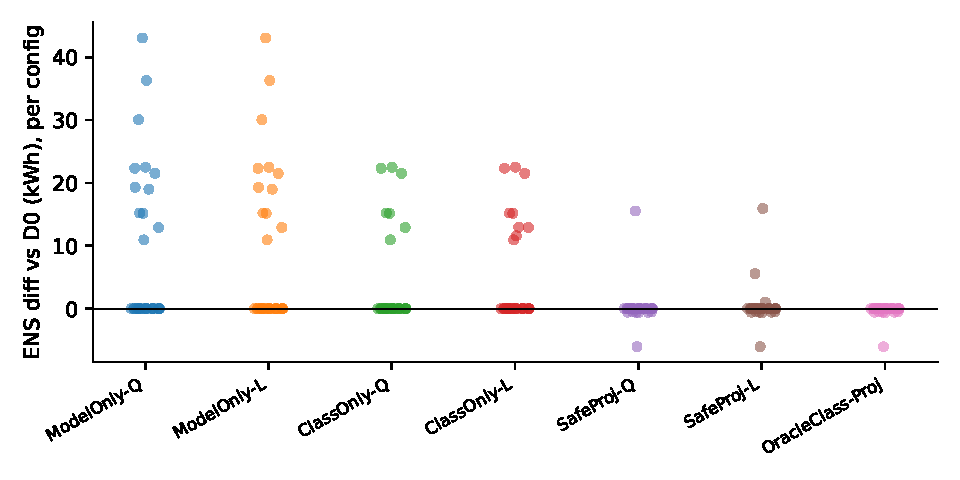
\includegraphics[width=\columnwidth]{figure/final_v3/fig_holdout_ens_diff.pdf}
  \caption{Per-configuration ENS difference versus the deterministic fast path
    (D0) on the independent 49-configuration holdout (paired CIs in
    Table~\ref{tab:stats-primary}). The projection arms (SafeProj-Q/SafeProj-L)
    sit near zero; the class-override arms sit above it; the ModelOnly arms
    (diagnostic, not matched ablations; \S\ref{sec:rq3}) sit highest.}
  \label{fig:holdout-v3}
\end{figure}

\begin{table}[t]
\centering\small
\caption{Horizon-aware estimator (EH) robustness: tie-aware top-1 optimal-action
rate and regret under horizon misspecification, delayed/partial execution, and
alternative cost weights, on the 12-configuration frozen estimator holdout. EH's
ranking is stable because the five-action choice is structurally determined;
point magnitudes remain imprecise (MAE $\approx$26\,kWh), so no
magnitude-prediction claim is made.}
\label{tab:eh-v3}
\begin{tabular}{lcccc}
\toprule
Condition & EH top-1 & EH med.\ regret & EH worst & E60 top-1 \\
\midrule
Nominal            & 1.00 & 0.00 & 0.0 & 0.33 \\
Horizon $-50\%$    & 1.00 & 0.00 & 0.0 & 0.33 \\
Horizon $-25\%$    & 1.00 & 0.00 & 0.0 & 0.33 \\
Horizon $+25\%$    & 1.00 & 0.00 & 0.0 & 0.33 \\
Horizon $+50\%$    & 1.00 & 0.00 & 0.0 & 0.33 \\
Delayed 10\,s      & 1.00 & 0.00 & 0.0 & 0.33 \\
Delayed 30\,s      & 1.00 & 0.00 & 0.0 & 0.33 \\
Partial failure    & 1.00 & 0.00 & 0.0 & 1.00 \\
$w_{\text{ENS}}=3$ & 1.00 & 0.00 & 0.0 & 0.33 \\
$w_{\text{ENS}}=8$ & 1.00 & 0.00 & 0.0 & 0.33 \\
\bottomrule
\end{tabular}
\end{table}


\subsection{RQ4: does the safety boundary hold under latency and fallback?}
\label{sec:rq4}
\emph{Experiment.} In deadline-aware mode the deterministic fast path acts at
detection; the model runs concurrently and its action replaces the fast-path
action only if it arrives within the service-level objective and passes every
safety check; an expired result never rewrites history. Measured per-call
latencies (Table~\ref{tab:latency-v3}) are replayed at SLOs of $1$--$60$\,s.

\emph{Result.} Single-call ($K{=}1$) inference is $5.45$\,s mean (Qwen) /
$5.62$\,s (Llama); $K{=}3$ self-consistency is $16.8$--$17.4$\,s and is not the
default. All latency values in the paper are regenerated from one measurement
file (Table~\ref{tab:latency-v3}). At a $1$\,s SLO no consultation lands
and the fast path stands alone; $K{=}1$ admits from $10$\,s (Qwen $0.99$, Llama
$1.00$), $K{=}3$ only from $30$\,s. Because the shield maps any accepted
proposal onto the same bounded primitive, physical outcomes are unchanged across
SLOs, and a late or failed model call deterministically leaves the fast-path
action in force under invariant~I5 (tested, not formally proved).
\emph{Interpretation.} The fast-path/slow-path split is an implementation-feasible
posture in the evaluated testbed: the model is advisory, and its absence
never removes containment. \emph{Limitation.} Latencies are single-GPU;
utility-grade serving changes constants, not the architecture.

\begin{table}[t]
\centering\small
\caption{Per-backbone, per-$K$ consultation-latency distribution, from the
146-call ($K{=}1$) / 48-call ($K{=}3$) measurements; single-call ($K{=}1$)
inference is $\approx$5.5\,s on both backbones. All latency values in the paper
are regenerated from this measurement file. Adapter load is a one-off startup
cost, not part of per-call latency.}
\label{tab:latency-v3}
\begin{tabular}{llccccccc}
\toprule
Backend & $K$ & $n$ & mean & median & s.d. & p95 & p99 & max \\
 & & & (s) & (s) & (s) & (s) & (s) & (s) \\
\midrule
Qwen & $K{=}1$ & 146 & 5.45 & 5.51 & 0.90 & 6.22 & 8.60 & 11.76 \\
Qwen & $K{=}3$ & 48 & 16.82 & 17.41 & 1.47 & 18.32 & 19.06 & 19.14 \\
Llama & $K{=}1$ & 146 & 5.62 & 5.60 & 0.57 & 6.56 & 7.03 & 8.34 \\
Llama & $K{=}3$ & 48 & 17.45 & 17.54 & 1.65 & 20.25 & 22.28 & 23.60 \\
\bottomrule
\end{tabular}
\end{table}


\section{Discussion}
\label{sec:discussion}

\subsection{What actually provides the safety}
\label{sec:disc-safety}
Across every experiment, deterministic mechanisms decide whether an unsafe action
reaches the feeder: the Evidence Gate decides whether anything may act, the
class-aware removals decide what may act, and the never-auto-execute rule
keeps a model-proposed irreversible primitive from executing autonomously. The ablation
localises containment almost entirely in the class-aware avoidance; components
that improve the \emph{model's} behaviour leave the \emph{system's} safety
unchanged, because safety was never delegated to the model. The trust boundary is
placed so the model's error rate multiplies into operator workload and advisory
quality, not physical consequence.

\subsection{What the LLM contributes --- and does not}
\label{sec:disc-llm}
The evaluated LLM advisers do not improve physical outcomes. The projection arms
show no statistically detectable difference from the deterministic fast path on
ENS and curtailment ($+0.19$ and $+0.40$\,kWh versus D0, both Holm $p=1.0$); of
the class-override arms, ClassOnly-L is worse after correction (Holm $p=0.041$)
while ClassOnly-Q is worse in point estimate but not significant (Holm
$p=0.107$); and the advisory path alone misses attacks the deterministic path
catches --- its in-loop classification is far below the deterministic evidence
mapping.
Crucially, the ground-truth-class oracle through the same shield \emph{is}
modestly better than the deterministic path ($-0.29$\,kWh, 95\% CI
$[-0.69, -0.05]$, excluding zero; raw $p=0.015$ but Holm-adjusted
$p=0.11$, so not significant after multiplicity correction). Two things
follow. There is a small amount of headroom that a \emph{correct}
classifier could capture, concentrated in the DoS cases where the
deterministic EH ranking already recovers most of it; and the evaluated
LLMs do not reach even that modest headroom. The result is not that
advisory quality is irrelevant, but that runtime projection contains
unsafe execution while leaving the model's contribution to physical
performance small and, for the models we tested, unrealised. What the model does
contribute is structured hypotheses, rationales for escalation, and an interface
for operator interrogation. The present evaluation establishes \emph{containment}
of the advisory model, not its operational utility: these outputs may support
operator-facing workflows, but their effect on operator accuracy, workload,
response time, and trust was not evaluated, and our groundedness audit
(70--73\% templated rationales, 23--30\% asserting evidence absent from the
input) shows the rationales are imperfect. Those benefits therefore remain
hypotheses for future human-subject study. The defensible conclusion is that
consultation can be isolated from direct execution authority within the tested
architecture; whether that consultation is operationally worthwhile remains
unestablished.

\subsection{Why model output must gate neither action nor inaction}
\label{sec:disc-confidence}
The two sharpest negative results are mirror images. A shield variant that
auto-executed an irreversible action on the model's stated confidence was worse
than no shield, because injection payloads manufacture exactly the
high-confidence prediction the gate keyed on; and a projection that honoured the
model's \textsc{no\_op} stood down a deterministically evidenced DoS, because the
attack shows the model a frozen copy of \emph{normal} telemetry --- the most
plausible input for ``no incident.'' In both directions the attacker does not
defeat the shield; it feeds the model. The rule is symmetric and, we believe,
load-bearing for any LLM-in-the-loop runtime assurance: \emph{no
attacker-influenceable quantity may relax a constraint on an irreversible action
or stand down a deterministically evidenced incident}. Confidence, rationale,
memory, predicted class, and proposed inaction all fail this test; protocol-level
evidence computed outside the model passes it.

\subsection{What the estimator episode teaches}
\label{sec:disc-estimator}
Counterfactual validation showed a plausible 60-second Energy Impact estimator
selected a tie-optimal action in only about a third of configurations, because it
was calibrated over a window on which the five primitives are nearly
indistinguishable while their true costs diverge over the incident horizon. The
repair needed no learning: the same physical priors, integrated over a
dev-calibrated estimate of the \emph{remaining incident duration} with
restoration-horizon accounting, rank optimally on the (small) held-out set. The
lesson is that impact estimators in response systems must be validated against
branched counterfactual rollouts \emph{at the horizon on which their decisions
bind}. A second point: decision-time identifiability limits matter less than they
appear --- replay and DoS cannot be distinguished when the whole telemetry
sample is stale, but the minimax action (\textsc{freeze\_setpoint}) is
optimal under one hypothesis and free under the other, so the ambiguity
need not be resolved to act well.

\subsection{What the evidence-provenance audit taught us}
\label{sec:disc-provenance}
A methodological point underlies the FDI result and generalises. A
tempting way to detect false-data injection in a simulator is to consult a
per-event flag that the attack generator itself sets; such a flag is
categorical and perfectly reliable, and it makes a gate look stronger than
any detector limited to observable evidence could be. We forbid it: every gate feature is
computed only from wire-observable telemetry (Table~\ref{tab:provenance}).
Under that discipline three families keep genuine protocol signatures
(command packets, sequence regression, timestamp staleness), but a
within-capacity FDI --- a reading that is wrong yet not physically
impossible --- has no observable hard signature, and we report FDI coverage
by magnitude and name redundant sensing as the missing ingredient. The
general lesson is that in a simulation-based security evaluation the
decisive audit is of \emph{where every runtime feature comes from}: a
feature sourced from generator ground truth can make an architecture appear
to solve a problem it has not. The runtime path uses no simulator attack labels
or generator ground truth; its wire-observable evidence nonetheless remains
forgeable wherever authentication or redundant sensing is absent, so we do not
claim the detector is as strong as its clean-signal coverage suggests.

\subsection{Can this run under realistic OT timing?}
\label{sec:disc-timing}
Yes, with a specific division of labour. The deterministic path ---
FeatureView, gate, shield --- adds sub-millisecond per-tick cost and
responds within one control tick of sustained evidence
(${\approx}5$\,s with the frozen persistence thresholds). Model
consultation costs ${\approx}5.5$\,s ($K{=}1$) on a consumer GPU, so it
lands within a 10\,s SLO and is skipped under tighter deadlines with no
loss of containment; $K{=}3$ ($\approx$17\,s) is not the default because
it misses even a 15\,s SLO. The gate also rations the model's exposure: relative to the ungated model-only
arms, benign-day consultations fall by more than 80\% (a descriptive comparison
of consultation counts on the 16 benign holdout configurations), saving inference
budget and reducing the model's exposure to attacker-controllable prompt content.
Under DoS the response is honest rather than flattering: the ungated pipeline's
apparent immunity in that family came from benign-day false freezes that happened
to pre-mitigate later attacks; the gated system pays a small measured ENS cost
for not false-acting
on every benign day.

\subsection{Limitations}
\label{sec:disc-limitations}
\begin{enumerate}
\item \textbf{Benchmark and simulation scope.} All cyber-physical
  results come from a StubFeeder co-simulation and static OpenDSS
  snapshot solves on IEEE 13/34-node feeders; no dynamic time-series
  study, no real feeder, no utility deployment. The StubFeeder's
  physics (nominal-dispatch rule, ENS threshold) is exactly the
  structure EH exploits; real-feeder EH would inherit real model error.
\item \textbf{Model and data scope.} One adapter pair (Qwen2.5-7B,
  Llama-3.1-8B) fine-tuned on one 200-example synthetic corpus;
  evaluation prompts are scenario-derived rather than human-annotated;
  results may not transfer to other backbones or corpora.
\item \textbf{Detection-layer scope, and the FDI observability limit.}
  The gate's observable protocol signatures (forged command packets, sequence
  regression, staleness, rating-plausibility residual) presuppose an
  instrumented protocol layer, and --- absent authentication --- are forgeable
  by a network attacker rather than hard proof of an attack. Under the observable-only feature set, a
  \emph{within-capacity} false-data-injection attack has no observable
  hard signature and is not separable from benign operation without a
  redundant measurement channel, which this simulator does not model;
  such FDI is missed (gate-open $0/1$ at medium and low magnitude).
  Benign protocol quirks (historian echo) remain unresolvable by the gate
  alone, and a stealthy attacker who forges \emph{internally consistent}
  protocol evidence is outside the evaluated threat suite.
\item \textbf{Empirical, not formal, assurance.} Zero-execution results
  are suite-bounded (95\% Clopper--Pearson upper bound $0.051$ on 70
  cases); the invariants are deterministic and directly testable but not
  formally proved, and an adaptive white-box adversary is not modelled.
\item \textbf{Human factors.} HITL operators are deterministic
  stand-ins. The observed escalation burden was strongly
  backbone-dependent (SafeProj-Q escalated 6 of 33 attack configurations,
  SafeProj-L none, because Qwen proposes the irreversible primitive far more
  often than Llama), but the available evaluation was not designed to establish
  the cause or the operational acceptability of that difference, and says
  nothing about real operator workload, fatigue, or trust.
\item \textbf{Auditability scope.} The audit chain provides append-only
  integrity verified by tamper tests, not cryptographic timestamping or
  a signature scheme.
\item \textbf{Drift and lifecycle.} Adapters, thresholds and the frozen
  gate calibration are point-in-time; concept drift, fleet
  reconfiguration, and adversary adaptation over time are unevaluated.
\end{enumerate}

\section{Conclusion}
\label{sec:conclusion}
We asked whether an unverified language model can be consulted safely
inside a cyber-physical incident-response path for distributed energy
resources, and answered with \ours: a runtime-assurance architecture in
which a deterministic Evidence Gate authorizes response when observable
evidence meets its frozen thresholds, a deterministic shield decides what may
execute, a model-proposed irreversible action is never auto-executed (vetoed
or escalated to a human), and a
validated horizon-aware estimator ranks the bounded fallback set --- while the
model contributes only bounded, auditable advice.

What the evidence supports: on a hash-frozen held-out set of configurations and a
canonical 70-case adversarial suite, all under a runtime-safe path that reads no
attack ground truth, deterministic projection contained unsafe autonomous
execution. The model is consulted on the large majority of adversarial cases, yet
the shielded architecture executed no autonomous irreversible action for either
backbone, compared with $61/70$ for the unshielded Qwen adviser and $18/70$ for
the unshielded Llama adviser; an exhaustive enumeration of the modelled decision
space ($40{,}824$ states) found no violation of the tested invariants, and
guard-removal mutations produced violations. The gate reduced benign-day false
mitigation while cutting the model's exposure to attacker-supplied prompt
content. The evaluated LLM advisers did not improve physical outcomes: the
projection arms show no statistically detectable difference from the
deterministic fast path, while a ground-truth-class oracle yielded only a modest
improvement (95\% CI excluding zero but not surviving multiplicity correction)
that the LLMs did not reproduce. The contribution is the execution boundary and
evidence discipline, not the model.

What it does not demonstrate: no formal guarantee, no real-feeder or utility
deployment, no human-operator study, and no robustness beyond the tested suite.
Gate detection remains limited by observability, authentication, and small
sample size; the zeros are suite-bounded estimates over the modelled space, not
proofs; wire-observable evidence stays forgeable where authentication or
redundant sensing is absent; and a within-capacity false-data-injection attack is
not detectable here without redundant sensing.

The lesson we believe outlives this system is twofold. First,
architectural: attacker-influenceable model output must relax no
constraint in either direction --- neither authorising an irreversible
action nor vetoing an evidenced incident --- and an LLM's place in
critical-energy-infrastructure response is inside a deterministic
envelope that makes its errors operationally cheap. Second,
methodological: in a simulation-based security study the decisive audit
is of \emph{where every runtime feature comes from}, because a feature
sourced from ground truth can make an architecture appear to solve a
problem it has not. The defensible contribution is the bounded action
surface and the evidence discipline around it, not the model that
proposes within it.

\section*{Code and Data Availability}
\begingroup\sloppy
The reproducibility package for this study is public at
\url{https://github.com/MyeongHaHwang/DER-SafeAgent} (release tag
\texttt{v1.1.0} is the version of record for the numbers reported here; the
repository's \texttt{CHANGELOG.md} and \texttt{RELEASE\_AUDIT.md} record the
verified state). The package contains the complete \ours{} implementation
--- the runtime-safe feature view, Evidence Gate, safety-projection shield,
estimators, fixed mitigation registry, and hash-chained audit record
(\texttt{code/Multi\_AI\_Agent/}), the strict local QLoRA serving layer
(\texttt{code/llm\_serving/}), the StubFeeder/OpenDSS simulation harness
with attack injectors (\texttt{code/simulation/}), baselines, and the
evaluation drivers (\texttt{code/evaluation/final\_safeagent\_v3/} is the
canonical pipeline) --- together with the safety-invariant and provenance
test suite, the machine-readable action-policy export behind
Table~\ref{tab:action-policy} (\texttt{code/configs/action\_policy.yaml}),
the hash-frozen experiment protocols (the 49-configuration end-to-end
holdout, the 32-configuration Evidence-Gate test set, the 12-configuration
estimator holdout, the development manifests, and the frozen gate operating
point), the canonical raw and processed result files behind every reported
table and figure, and the manuscript LaTeX source. Every released
configuration, dataset, adapter, and result artifact is identified by a
SHA-256 digest in the package manifests
(\texttt{data/manifests/}), an included verification script re-checks all
digests, and \texttt{docs/PAPER\_ARTIFACT\_MAP.md} maps each table and
figure to its source data and generation script; a claim-by-claim audit of
the reported numbers is kept in \texttt{docs/CLAIM\_LEDGER.md}. The numeric
tables and figures of this paper regenerate from the canonical result files
on a CPU-only machine with a single command (\texttt{make reproduce-paper}),
without re-running any model inference.

The synthetic v0.1 fine-tuning corpus (200 examples; 161/21/18
train/val/test split) is released under
\texttt{code/finetuning\_dataset/processed/} with per-row SHA-256 hashes,
alongside the leakage-controlled evaluation corpus and the generator of the
70-case adversarial suite. The QLoRA adapters used in all experiments are
released (via Git LFS) with their training configurations, prompt hashes,
and adapter checksums; the Qwen2.5-7B-Instruct and Llama-3.1-8B-Instruct
base weights are not redistributed and must be obtained separately under
their original licenses. Full model-in-the-loop re-execution requires a
single NVIDIA GPU ($\geq$10\,GB VRAM with 4-bit quantization) and the
software environment documented in the package; CPU-only commands cover the
safety tests, artifact integrity verification, and regeneration of the
reported tables and figures. The UNSW-MG24 and TON\_IoT datasets and per-run
holdout trace dumps are not redistributed; loader code, a synthetic mock
fixture, and acquisition instructions are included, and every emitted result
row records its \texttt{result\_source} so mock- and production-derived rows
cannot be conflated. All DER measurements and attack scenarios in this study
are synthetic or simulation-derived (StubFeeder episodes and static IEEE
13/34-bus OpenDSS power-flow snapshots); no personal data and no operational
utility credentials are included. A naming note: the system was renamed from
\textsc{DER-SecAgent} to \ours{}; package and result directories retain the
legacy name to preserve the recorded configuration hashes.
\par\endgroup


%% --------------------------------------------------------------------------
%%  References --- elsarticle-num style for IJCIP
%% --------------------------------------------------------------------------
\bibliographystyle{elsarticle-num}
\bibliography{sections/References}

%% Appendix material has moved to the separate supplementary document
%% (paper/supplementary.tex, S1--S10), per the final revision.

\end{document}
